%%%%%%%%%%%%%%%%%%%%%%%%%%%%%%%%%%%%%%%%%%%%%%%%%%%%%%%%%%%%%%%%%%%
%                                                                 %
%                            ROOT FILE                            %
%                                                                 %
%%%%%%%%%%%%%%%%%%%%%%%%%%%%%%%%%%%%%%%%%%%%%%%%%%%%%%%%%%%%%%%%%%%
%
%  Run LaTeX or pdfLaTeX on this file to produce your thesis.
%  To produce the abstract title page followed by the abstract,
%  see the file abstitle-phd.tex or abstitle-mas.tex.
%
%%%%%%%%%%%%%%%%%%%%%%%%%%%%%%%%%%%%%%%%%%%%%%%%%%%%%%%%%%%%%%%%%%%

\documentclass[chap]{thesis}

%%%%%%%%%%%%%%%%%%%%%%%%%%%%%%%%%%%%%%%%%%%%%%%%%%%%%%%%%%%%%%%%%%%

\usepackage{graphicx}
%\usepackage{amsmath}
%\usepackage{amsthm}
%\usepackage{amssymb}
\usepackage[usenames,dvipsnames,svgnames,table]{xcolor}
\usepackage{pdfpages}
\usepackage{tikz}
\usepackage{amsmath}
\usepackage{amssymb}
\usepackage[numbers]{natbib}
\usepackage[labelfont=bf]{caption}
\usepackage[labelformat=simple]{subfig}
\usepackage{mathtools}

\DeclarePairedDelimiter\ceil{\lceil}{\rceil}
\DeclarePairedDelimiter\floor{\lfloor}{\rfloor}

\newcommand*{\head}[1]{%
	\textbf{#1}
}
\newcommand{\cnote}[1]{%
	{\color{red}[#1]}
}
\renewcommand{\textfraction}{0.01}
\renewcommand{\floatpagefraction}{0.99}
\renewcommand{\topfraction}{0.99}
\renewcommand{\bottomfraction}{0.99}
\renewcommand{\dblfloatpagefraction}{0.99}
\renewcommand{\dbltopfraction}{0.99}
\renewcommand{\th}{$^{th}$}
\newcommand{\conv}{\mathop{\scalebox{1.2}{\raisebox{-0.2ex}{$\ast_{x,y}$}}}}

%%%%%%%%%%%%%%%%%%%%%%%%%%%%%%%%%%%%%%%%%%%%%%%%%%%%%%%%%%%%%%%%%%%

\begin{document}

    %%%%%%%%%%%%%%%%%%%%%%%%%%%%%%%%%%%%%%%%%%%%%%%%%%%%%%%%%%%%%%%%%%%
%                                                                 %
%                            TITLE PAGE                           %
%               Master's Thesis or Master's Project               %
%                                                                 %
%%%%%%%%%%%%%%%%%%%%%%%%%%%%%%%%%%%%%%%%%%%%%%%%%%%%%%%%%%%%%%%%%%%

% Supply information for use on title page:
\thesistitle{\bf Photographic Censusing of Zebra and Giraffe in the Nairobi National Park}
\author{Jason R.\ Parham}
\degree{Master of Science}
\department{Computer Science}

\signaturelines{3}
\projadviser{Dr. Charles Stewart}
\memberone{Dr. Barbara Cutler}
\membertwo{Dr. B{\"u}lent Yener}

\submitdate{November 2015\\(For Graduation December 2015)}
\copyrightyear{2015}   % if omitted, current year is used.

% Print titlepage and other prefatory material:
\titlepage
\copyrightpage         %optional
\tableofcontents
\listoftables          %required if there are tables
\listoffigures         %required if there are figures


    \newpage

    %%%%%%%%%%%%%%%%%%%%%%%%%%%%%%%%%%%%%%%%%%%%%%%%%%%%%%%%%%%%%%%%%%%
%                                                                 %
%                         ACKNOWLEDGEMENTS                         %
%                                                                 %
%%%%%%%%%%%%%%%%%%%%%%%%%%%%%%%%%%%%%%%%%%%%%%%%%%%%%%%%%%%%%%%%%%%

\specialhead{ACKNOWLEDGMENTS}

\textit{The Great Zebra \& Giraffe Count} (GZGC) was powered and administered by the IBEIS team with notable help from Dr.\ Paula Kahumbu and staff at Wildlife Direct in Nairobi, Kenya.  The IBEIS team would like to thank the people and government of Kenya for supporting this research (Permit \# NACOSTI/P/14/1003/1628), with special recognition to Senior Warden of the Nairobi National Park, Nely Palmeris, and Macharia ``Michael'' Kimura of the Kenyan Wildlife Service (KWS).  Other contributions to this thesis were provided by Clara Machogu, Marco Maggioni, Jon Crall, Hendrik Weideman, Michael Brown, and Zachary Jablons.  I would like to thank Dr.\ Tanya Berger-Wolf, Dr.\ Daniel Rubenstein, and my master committee members, Dr.\ Barbara Cutler and Dr.\ B{\"u}lent Yener, for their valuable feedback.  I would also like to give a special thank you to my Ph.D.\ advisor, Dr.\ Charles Stewart, who has patiently guided me to this milestone of my academic career.

All of the software detailed in this thesis can be downloaded from open-source code repositories.  The IBEIS software can be downloaded on GitHub \footnote{github.com/erotemic/ibeis [Accessed: Nov. 1, 2015]} and the client-server code used during the GZGC data collection event can also be downloaded on Github \footnote{github.com/bluemellophone/[gzc-client, gzc-server] [Accessed: Nov. 1, 2015]}.  The open-source software and research detailed in this thesis was supported by Rensselaer Polytechnic Institute (RPI) and with financial support from NSF EAGER Grant (Award \#1453503) \textit{Collaborative Research: EAGER: Prototype of an Image-Based Ecological Information System (IBEIS)}.

Lastly, but most importantly, I would like to thank my wife, Lindsay, for providing patient, never-failing support.  Her dedication to my academic career and intellectual progress has been the best example of sacrificial love I have ever had the privilege to personally experience.

\begin{figure}[!htb]%
    \centering
    \subfloat {{ $\vcenter{\hbox{ \includegraphics[height=0.15\textwidth]{resources/logo_ibeis.png} }}$ }}%
    \qquad
    \subfloat {{ $\vcenter{\hbox{ \includegraphics[height=0.12\textwidth]{resources/logo_wd_alpha.png} }}$ }}%
\end{figure}


    \newpage

    \input{rpiabs}
    %%%%%%%%%%%%%%%%%%%%%%%%%%%%%%%%%%%%%%%%%%%%%%%%%%%%%%%%%%%%%%%%%%%
%                                                                 %
%                            CHAPTER ONE                          %
%                                                                 %
%%%%%%%%%%%%%%%%%%%%%%%%%%%%%%%%%%%%%%%%%%%%%%%%%%%%%%%%%%%%%%%%%%%

\chapter{INTRODUCTION} \label{sec:introduction}

How many plains zebras (\textit{Equus quagga}) and Masai giraffes (\textit{Giraffa camelopardalis tippelskirchi}) are in the Nairobi National Park?

The question, at its surface, may seem trivial -- a two year old child can reliably count zebras and giraffes -- but the answer becomes difficult to obtain when the population becomes unmanageable.  To be more precise, the unmanageability originates when either the conservation area is too large to be effectively and efficiently sampled, the population grows to a point that exceeds the conservationists' ability to keep reliable records of the different individuals, or both.  At that point, finding the answer becomes intractable for human-powered identification and analysis.  For the Nairobi National Park, the problem is further complicated by the fact that the park is not fenced on its southern side -- it is typical of most conservancies in Kenya to have an unfenced boundary to prevent limiting natural migration -- making the actual zebra and giraffe population arbitrary at any particular moment, and ever-changing.  Therefore, merely locating the zebras within the park and producing a representative sampling of the population is a significant obstacle.

%\begin{figure*}[t]%
\begin{figure}[!htb]%
    \centering
    \subfloat[]{{ $\vcenter{\hbox{ \includegraphics[width=0.215\textwidth]{resources/matching/1-667-2.jpeg} }}$ }}%
    \subfloat[]{{ $\vcenter{\hbox{ \includegraphics[width=0.215\textwidth]{resources/matching/10-229-1.jpeg} }}$ }}%
    \subfloat[]{{ $\vcenter{\hbox{ \includegraphics[width=0.215\textwidth]{resources/matching/11-253-2.jpeg} }}$ }}%
    \subfloat[]{{ $\vcenter{\hbox{ \includegraphics[width=0.215\textwidth]{resources/matching/12-2773-2.jpeg} }}$ }}%
    \vspace{0.1cm}
    \subfloat[]{{ $\vcenter{\hbox{ \includegraphics[width=0.215\textwidth]{resources/matching/13-3039-2.jpeg} }}$ }}%
    \subfloat[]{{ $\vcenter{\hbox{ \includegraphics[width=0.215\textwidth]{resources/matching/14-229-2.jpeg} }}$ }}%
    \subfloat[]{{ $\vcenter{\hbox{ \includegraphics[width=0.215\textwidth]{resources/matching/15-236-1.jpeg} }}$ }}%
    \subfloat[]{{ $\vcenter{\hbox{ \includegraphics[width=0.215\textwidth]{resources/matching/16-3039-1.jpeg} }}$ }}%
    \vspace{0.1cm}
    \subfloat[]{{ $\vcenter{\hbox{ \includegraphics[width=0.215\textwidth]{resources/matching/17-3250-2.jpeg} }}$ }}%
    \subfloat[]{{ $\vcenter{\hbox{ \includegraphics[width=0.215\textwidth]{resources/matching/18-667-1.jpeg} }}$ }}%
    \subfloat[]{{ $\vcenter{\hbox{ \includegraphics[width=0.215\textwidth]{resources/matching/19-2773-1.jpeg} }}$ }}%
    \subfloat[]{{ $\vcenter{\hbox{ \includegraphics[width=0.215\textwidth]{resources/matching/2-56-1.jpeg} }}$ }}%
    \vspace{0.1cm}
    \subfloat[]{{ $\vcenter{\hbox{ \includegraphics[width=0.215\textwidth]{resources/matching/20-3250-1.jpeg} }}$ }}%
    \subfloat[]{{ $\vcenter{\hbox{ \includegraphics[width=0.215\textwidth]{resources/matching/3-212-1.jpeg} }}$ }}%
    \subfloat[]{{ $\vcenter{\hbox{ \includegraphics[width=0.215\textwidth]{resources/matching/4-253-1.jpeg} }}$ }}%
    \subfloat[]{{ $\vcenter{\hbox{ \includegraphics[width=0.215\textwidth]{resources/matching/5-212-2.jpeg} }}$ }}%
    \vspace{0.1cm}
    \subfloat[]{{ $\vcenter{\hbox{ \includegraphics[width=0.215\textwidth]{resources/matching/6-583-1.jpeg} }}$ }}%
    \subfloat[]{{ $\vcenter{\hbox{ \includegraphics[width=0.215\textwidth]{resources/matching/7-236-2.jpeg} }}$ }}%
    \subfloat[]{{ $\vcenter{\hbox{ \includegraphics[width=0.215\textwidth]{resources/matching/8-56-2.jpeg} }}$ }}%
    \subfloat[]{{ $\vcenter{\hbox{ \includegraphics[width=0.215\textwidth]{resources/matching/9-583-2.jpeg} }}$ }}%
    \vspace{0.1cm}
    \caption[Matching Game for Pairs of 10 Individual Zebras]{\textbf{Matching Game for Pairs of 10 Individual Zebras.}  A game to match the pairs (2 images per animal) of 10 identified individuals seen during the GZGC.    Answers can be found in Table \ref{tab:answers} in the Appendix.  Once completed, we suggest the reader reflect on the follwing questions: 1) ``How confident are you in your matches?'' 2) ``How difficult was the appearance-based matching?'' 3) ``How long did it take?'' and 4) Using the answers, ``How accurate were your matches?''}
        \label{fig:matching}
\end{figure}

The intractability is not as much of a concern for larger or endangered species such as elephants and rhinoceroses, where a small, local population can be manageably and reliably identified using ear notches and tags \cite{mukinya_identification_1976}, radio collars \cite{alexander_african_1994, mech_critique_2002, thouless_long_1995}, or other physical distinguishing features (e.g.\ deformities, scars, face shape, ear shape and wrinkles) \cite{patrick_demographic_2003, sikes_guidelines_2011}.   However, most of these approaches are \textit{invasive} and require involved procedures, such as incapacitating the animal using expensive tranquilizers and employing experienced veterinarians.  A better approach to estimating the animal population would be to simply use the appearance of the animal to \textit{passively} (non-invasively) identify the individual.  For large populations of zebra or giraffe, or even large populations of elephant or rhinoceros, the cost and demanding logistics makes invasively identifying the population infeasible.  Therefore, a passive, appearance-based approach is preferred.  However, it is exceedingly difficult for humans to reliably distinguish between different individual animals based solely on unaltered appearance \cite{crall_hotspotter_2013} without added identifying markers.  To illustrate this, we have provided an example of 20 images of zebras in Figure \ref{fig:matching}.  We invite the reader to spend (at most) 10 minutes examining and to attempt matching the image pairs (2 images per animal) for 10 identified individuals.  These sightings of zebra were selected from the population at the Nairobi National Park.  The purpose of the matching game is to highlight the uncertainty, difficulty, and duration of matching between different sightings of zebras.  For brevity, the discussion in this thesis will focus largely on plains zebras since the procedure and concepts are identical between zebras and giraffes.  We will revisit Masai giraffes in Chapter \ref{sec:results}.

Despite these challenges, it is still important for the conservationists to have an accurate estimate of the zebra population within the park.  Knowing the number of zebras can be used to measure the overall health of the park's ecosystem and can be used to help answer ecological questions, such as: ``is the population stable and self-sustaining?''\ \cite{andersen_population_2015, boyce_population_1992, coulson_use_2001, macedo_ecology_2010}, ``what are the population's age and sex demographics?''\ \cite{romer_population_2015, macedo_ecology_2010}, ``what is the life-expectancy?''\ \ \cite{romer_population_2015, macedo_ecology_2010, white_program_1999}, ``what is the impact of the population on the park's environment?''\ \cite{keesing_impacts_1998, macedo_ecology_2010}, and -- with GPS data -- ``what are the migratory patterns and locations of concentration?''\ \cite{karanth_estimating_2012, subedi_population_2013}.  The answers to these questions can be used by the conservationists to make data-driven decisions to better coordinate and focus their conservation efforts.  Up until now, estimates of the population in the Nairobi National Park were performed by simply counting sighted individuals within sub-sections of the park on a given day (e.g.\ \cite{oconnell_abundance_2011, seber_estimation_1982, subedi_population_2013}) or by counting from aerial surveys (e.g.\ \cite{caughley_sampling_1977, melville_aerial_2008, zero_monitoring_2013}). These counting-based procedures are prone to errors such as double counting, under-sampling, and sampling bias \cite{buckland_quantifying_1991, graham_investigating_1989, jachmann_comparison_2002, jolly_problem_1983, robson_sample_1964}.  A better system for producing a population estimate is therefore desired.  In this thesis, we present an alternate population counting method by implementing a distributed, automated, appearance-based approach to address these challenges and ultimately provide conservationists with the data they require.

To address the difficulty of sampling a large population and having to survey a large conservation area, we propose employing the help of volunteer participants.  The volunteers are tasked with photographing every zebra they encounter in an assigned zone (sub-section) within the conservation area, which provides input to a computer vision algorithm.  It is important to note that while the scientific contributions of these volunteers can be critical to a population estimate, the process should also be engaging and rewarding for these participants.  These so-called \textit{citizen scientists} \cite{cohn_citizen_2008, haklay_geographical_2010, sui_citizen_2013, irwin_citizen_1995, silvertown_new_2009} can be deputized for data collection and can thus significantly reduce the demands of performing a park-wide population monitoring study, freeing logistical man-power for other administrative duties.  If a large sampling of images is obtained, the challenge of estimating the zebra population is reformulated from an individual, human-powered identification and analysis problem into a highly-distributed, semi-automated, appearance-based process that uses images contributed by citizen scientists as input.  It should be mentioned that compared to camera traps, trail cameras, and automated camera drones, enlisting the help of citizen scientists is logistically simpler (e.g.\ no need to setup, monitor, and retrieve cameras) and obviously does not require purchasing additional hardware.  The images taken by a human photographer are generally of superior quality since a volunteer can be trained to take only useful pictures.  These benefits, however, come at the cost of having to incentivize citizen scientist involvement.   The involvement of citizen scientists also introduces sampling biases (e.g.\ trail cameras and camera traps capture images during night whereas volunteers might not).  An unbiased population monitoring study should use many sources of image input as can be reasonably obtained, however we only utilized images taken by citizen scientists for our sampling.

To address the inaccuracies and inefficiencies of human-powered, appearance-based identification, we propose leveraging the computational power of computer vision algorithms to help with tedious and high-volume tasks.  The computer vision algorithms are a starting point for beginning to automatically answer the following questions:
\begin{enumerate}
    \item Given an image, where are all of the zebras located?  % The computer vision answer is object detection and localization.
    \item Given a sighting of a zebra, is it of sufficient quality (e.g.\ exposure, focus, etc.)\ for identifying that individual?  % The computer vision answer is using scene features (GIST descriptors)
    \item Given a sighting of a zebra, how does its appearance describe that individual's identity?  Furthermore, is the description of sufficient quality to recognize that individual in the future?  % The computer vision answer is feature extraction.
    \item Given a zebra's description, has that individual zebra ever been seen previously?  % The computer vision answer is object recognition.
\end{enumerate}
The computer vision algorithms used in this thesis offer enough aid to make passive, appearance-based population monitoring feasible for large populations.

In the past, tedious appearance-based techniques were developed for estimating the size of an animal population.  Starting in the 1980's, film photographs were taken of animals and developed on-location to produce image negatives.  Using the negatives, the animal's stripes and visual patterns were traced onto paper by hand and a location-specific bifurcation tree was generated for identifying the known individuals  \cite{ginsberg_social_1988}.  This process was very resource intensive, had problems scaling to larger populations, and relied heavily on taking clear images from fixed viewpoints.  In the mid-1990's, software solutions for indexing the population began to emerge.  Using the encoding method described by Ginsberg \cite{ginsberg_social_1988}, the appearance of the animal was encoded into a (mostly) deterministic and searchable identification tag.  To query an animal, a regular expression search was used to find matching candidate images that were associated with a similar identification tag.  While much faster than the previous method, errors in determining the identification tag made the system difficult to use without rather extensive biological experience.  In the early 2000's, software developed by Hiby et al.  \cite{hiby_computer_1990, hiby_analysis_2013} allowed for a more sophisticated identification database to be created using visual \textit{guide dots}, which further improved the accuracy of searching but the required annotating of the algorithm's features was labor-intensive and slow.  As faster computers and more advanced computer vision algorithms became available, new algorithms (e.g.\ StripeSpotter \cite{lahiri_biometric_2011} and HotSpotter \cite{crall_hotspotter_2013}) succeeded in reducing or eliminating the amount of manual annotation required before performing a search in an identification data structure.  Our overall approach is very similar in structure and technical application to the work of Bolger et. al. \cite{bolger_computer-assisted_2012}, which was a computer-assisted ``photographic mark-recapture'' technique developed independently of our system.  Their culminating interface, called \texttt{Wild-ID}, and overall algorithm (while less sophisticated than our current software prototype) still achieved impressive results for Masai giraffes in northern Tanzania.

Previously, the most current and accurate population estimates for the zebra and giraffe populations in the Nairobi National Park were based on \textit{counting} methods.  In contrast, the population estimate described in this thesis is based on performing a \textit{photographic censusing}, or photographic mark-recapture (PMR)\cite{bolger_computer-assisted_2012} study, of the population.  The primary difference between counting and photographic censusing is that counting does not take into consideration resighted animals nor does it have the capability to capture fine-grained ecological data for individuals within the population (e.g.\ life-expectancy, individual movement, etc.).  A photographic censusing of the population, however, is able to recognize a resighted animal based on its appearance and produce more accurate ecological statistics for that individual and the population as a whole.  The most recent population count (2011) based on counting methods for plains zebras in the Nairobi National Park estimated 1000 - 2000 individuals and 100 individuals for Masai giraffes \cite{ogutu_changing_2013}.  While these estimates were performed annually or semi-annually, they do not provide continuous information, are a logistical and financial burden on the park administrators, and - since they do not capture individual-level information - do not accurately account for population changes due to birth, death, migration, or immigration.  One of the main contributions of this paper is to provide an appearance-based census of the zebra and giraffe populations within the Nairobi National Park which is robust by monitoring the sightings of individual animals over time.

In March of 2015, we administered a two-day data collection event entitled \textit{The Great Zebra \& Giraffe Count} (GZGC) during the \textit{Kenya Wildlife Festival} in Nairobi, Kenya.  The GZGC employed the help of volunteer citizen scientists to help collect image data and was powered by the IBEIS computer vision system; IBEIS is a Python-based, computer vision pipeline, based on the HotSpotter \cite{crall_hotspotter_2013} recognition algorithm.  During the GZGC, IBEIS semi-automatically\footnote{meaning it automatically offered weighted results that had to be reviewed} localized the animal in the image, filtered detections based on quality, described the animal, used the description to build and search a database for potential matches, verified the matches, aggregated the matches into a final weighted score, and semi-automatically used the final score to decide if the animal has been seen previously \cite{gall_class-specific_2009, lowe_distinctive_2004, muja_fast_2009}.  To our knowledge, this is the first time a population estimate of the plains zebras and Masai giraffes \footnote{IBEIS is designed to process many different species and is not limited to just zebras or giraffes.} has ever been performed using an automated appearance-based approach.  We also believe that the GZGC was the largest citizen science data collection event ever performed inside the park, to date.

This thesis describes the technical aspects of the citizen science data collection and the resulting analysis generated by using a prototype version of IBEIS.  Since the IBEIS prototype was incomplete, and the volume of data contributed during the GZGC was large, we needed to develop additional interfaces for efficient image submission and distributed reviewing of the results generated by the computer vision algorithms.  We also developed several innovative computer vision algorithms to replace human-powered annotating with automated tools for the next version of IBEIS and future population counting events.  The remaining chapters of this thesis describe the specific details of our approach used during the GZGC and the results, as follows.  Chapter \ref{sec:collection} describes the data collection and citizen scientist participation.  Chapter \ref{sec:analysis} details the analysis performed on the collected data using IBEIS.  Chapter \ref{sec:verification} covers the verification performed on the analysis.  Chapter \ref{sec:results} reports the results and the estimated zebra population in the park.  Finally, Chapter \ref{sec:conclusion} summarizes our results and concludes by giving future suggestions for improvements.

As a final introductory comment, we note that IBEIS is a large and complex system, with many contributors, and is far too expansive to comprehensively describe in a single Master's thesis.  Therefore, this thesis focuses on the author's current -- and somewhat-disjoint -- contributions to IBEIS and its usage during the GZGC.  Future Ph.D. dissertations will describe the major computer vision contributions and detailed aspects of the full IBEIS computer vision architecture.

\paragraph{Terminology}
We will refer to the Nairobi National Park as NNP, \textit{The Great Zebra \& Giraffe Count} as GZGC, and the prototype \textit{Image Based Ecological Information System} as IBEIS.

    %%%%%%%%%%%%%%%%%%%%%%%%%%%%%%%%%%%%%%%%%%%%%%%%%%%%%%%%%%%%%%%%%%%
%                                                                 %
%                            CHAPTER TWO                          %
%                                                                 %
%%%%%%%%%%%%%%%%%%%%%%%%%%%%%%%%%%%%%%%%%%%%%%%%%%%%%%%%%%%%%%%%%%%

\chapter{COLLECTION} \label{sec:collection}

\begin{figure*}[t]%
    \centering
    \subfloat {{ $\vcenter{\hbox{ \includegraphics[width=0.75\textwidth]{resources/printout.jpg} }}$ }}%
    \caption[Example Printout Returned to Each Citizen Scientist]{\textbf{Example Printout Returned to Each Citizen Scientist.}  Each participating citizen scientist recieved a printout showing a map of where the car drove (in blue) and information for three animals seen by that photographer (black, red, and green).  The other sightings for the three animals were also marked on the map.  This was the printout that was given to citizen scientist ``A'' in car ``8 WHITE''.  This participant saw one new animal (red) and resighted two animals (black and green).  The pictures taken by the participant are shown on the left and the matching animal (or information on the new sighting) is shown on the right.  The recognition matches were provided by IBEIS using an initial database.}
        \label{fig:printout}
\end{figure*}

Every citizen scientist who volunteered for the GZGC was first registered and then sent out into the NNP to collect image data.  After they completed their collection, all participants returned to the registration site so that their collected image data could be contributed, and subsets could be processed on-site.  The processing software used during the GZGC was developed as a client-server model (connected using a local, offline network); import client machines copied the image data    camera memory cards and then submitted them to a central server for processing.  Each participating citizen scientist received a printout showing a brief, preliminary analysis of the images they took.  An example printout can be seen in Figure \ref{fig:printout}.  The volume of collected data was too large relative to the processing capabilities of the system for more detailed feedback the day of collection.  All of the import client machines and the central processing server were laptop computers and needed to work without Internet connectivity to process the images.  The central IBEIS server laptop was a 64-bit AMD quad-core Lenovo laptop with 16 GB of RAM running Ubuntu 14.04.  The on-site data collection steps are described in more detail in the remainder of this chapter and are summarized in Figure \ref{fig:process}.

%Given this workflow, the GZGC operated under the following constraints and assumptions:
%\begin{enumerate}
%   \item The automatic or manual processing of the collected data was computationally intensive,
%   \item The collection protocol training for the citizen scientist needed to be minimal and be taught in a short period of time (5-15 minutes),
%   \item A small, uniform random sampling of the data collected by the citizen scientist was sufficient to summarize their entire data as a whole,
%   \item A participating citizen scientist was required to bring their own transportation and a personal camera with a removable memory card,
%   \item A participating citizen scientist expected some level of immediate feedback from the data they had collected that day, and
%   \item The processing of the collected data had to be agnostic to input order.
%\end{enumerate}

%For the GZGC,IBEIS producing the computer vision analytics was constrained by the efficiency of algorithms and the computational power of the server laptop;  on average, IBEIS could process an image, on average, in a few seconds.  Due to this processing bottleneck, immediate on-site processing of \textit{all} images collected by a citizen scientist was computationally infeasible; the semi-automatic results of detection and identification had to be manually reviewed.  This review process was ultimately a limiting man-power bottleneck that could have severely impacted the responsiveness of the GZGC if we had processed all images collected by a citizen scientist immediately and on-site.

%This chapter describes how image data was gathered and saved from the citizen scientist, sampled a small set of images for processing, processed the small image set by IBEIS, and then generated a printout result for the citizen scientist to keep.  It should be explicitly mentioned that the printout is critical to the success of the overall data collection;  the printout provides each citizen scientist with a reason to continue participate in future data collections as it is tangible proof of their contributions being utilized for some scientific goal, but also unctions as a potential marketing flier to facilitate the recruitment of future citizen scientists.  The time from when the citizen scientist returned with collected image data to when the printout was generated was 2 to 5 minutes, depending on the number of images collected by that citizen scientist and the processing load on the server at the time that individual returned.  An overview of the collection process can be viewed in Figure \ref{fig:process}.

\begin{figure*}[t]%
    \centering
    \subfloat {{ $\vcenter{\hbox{ 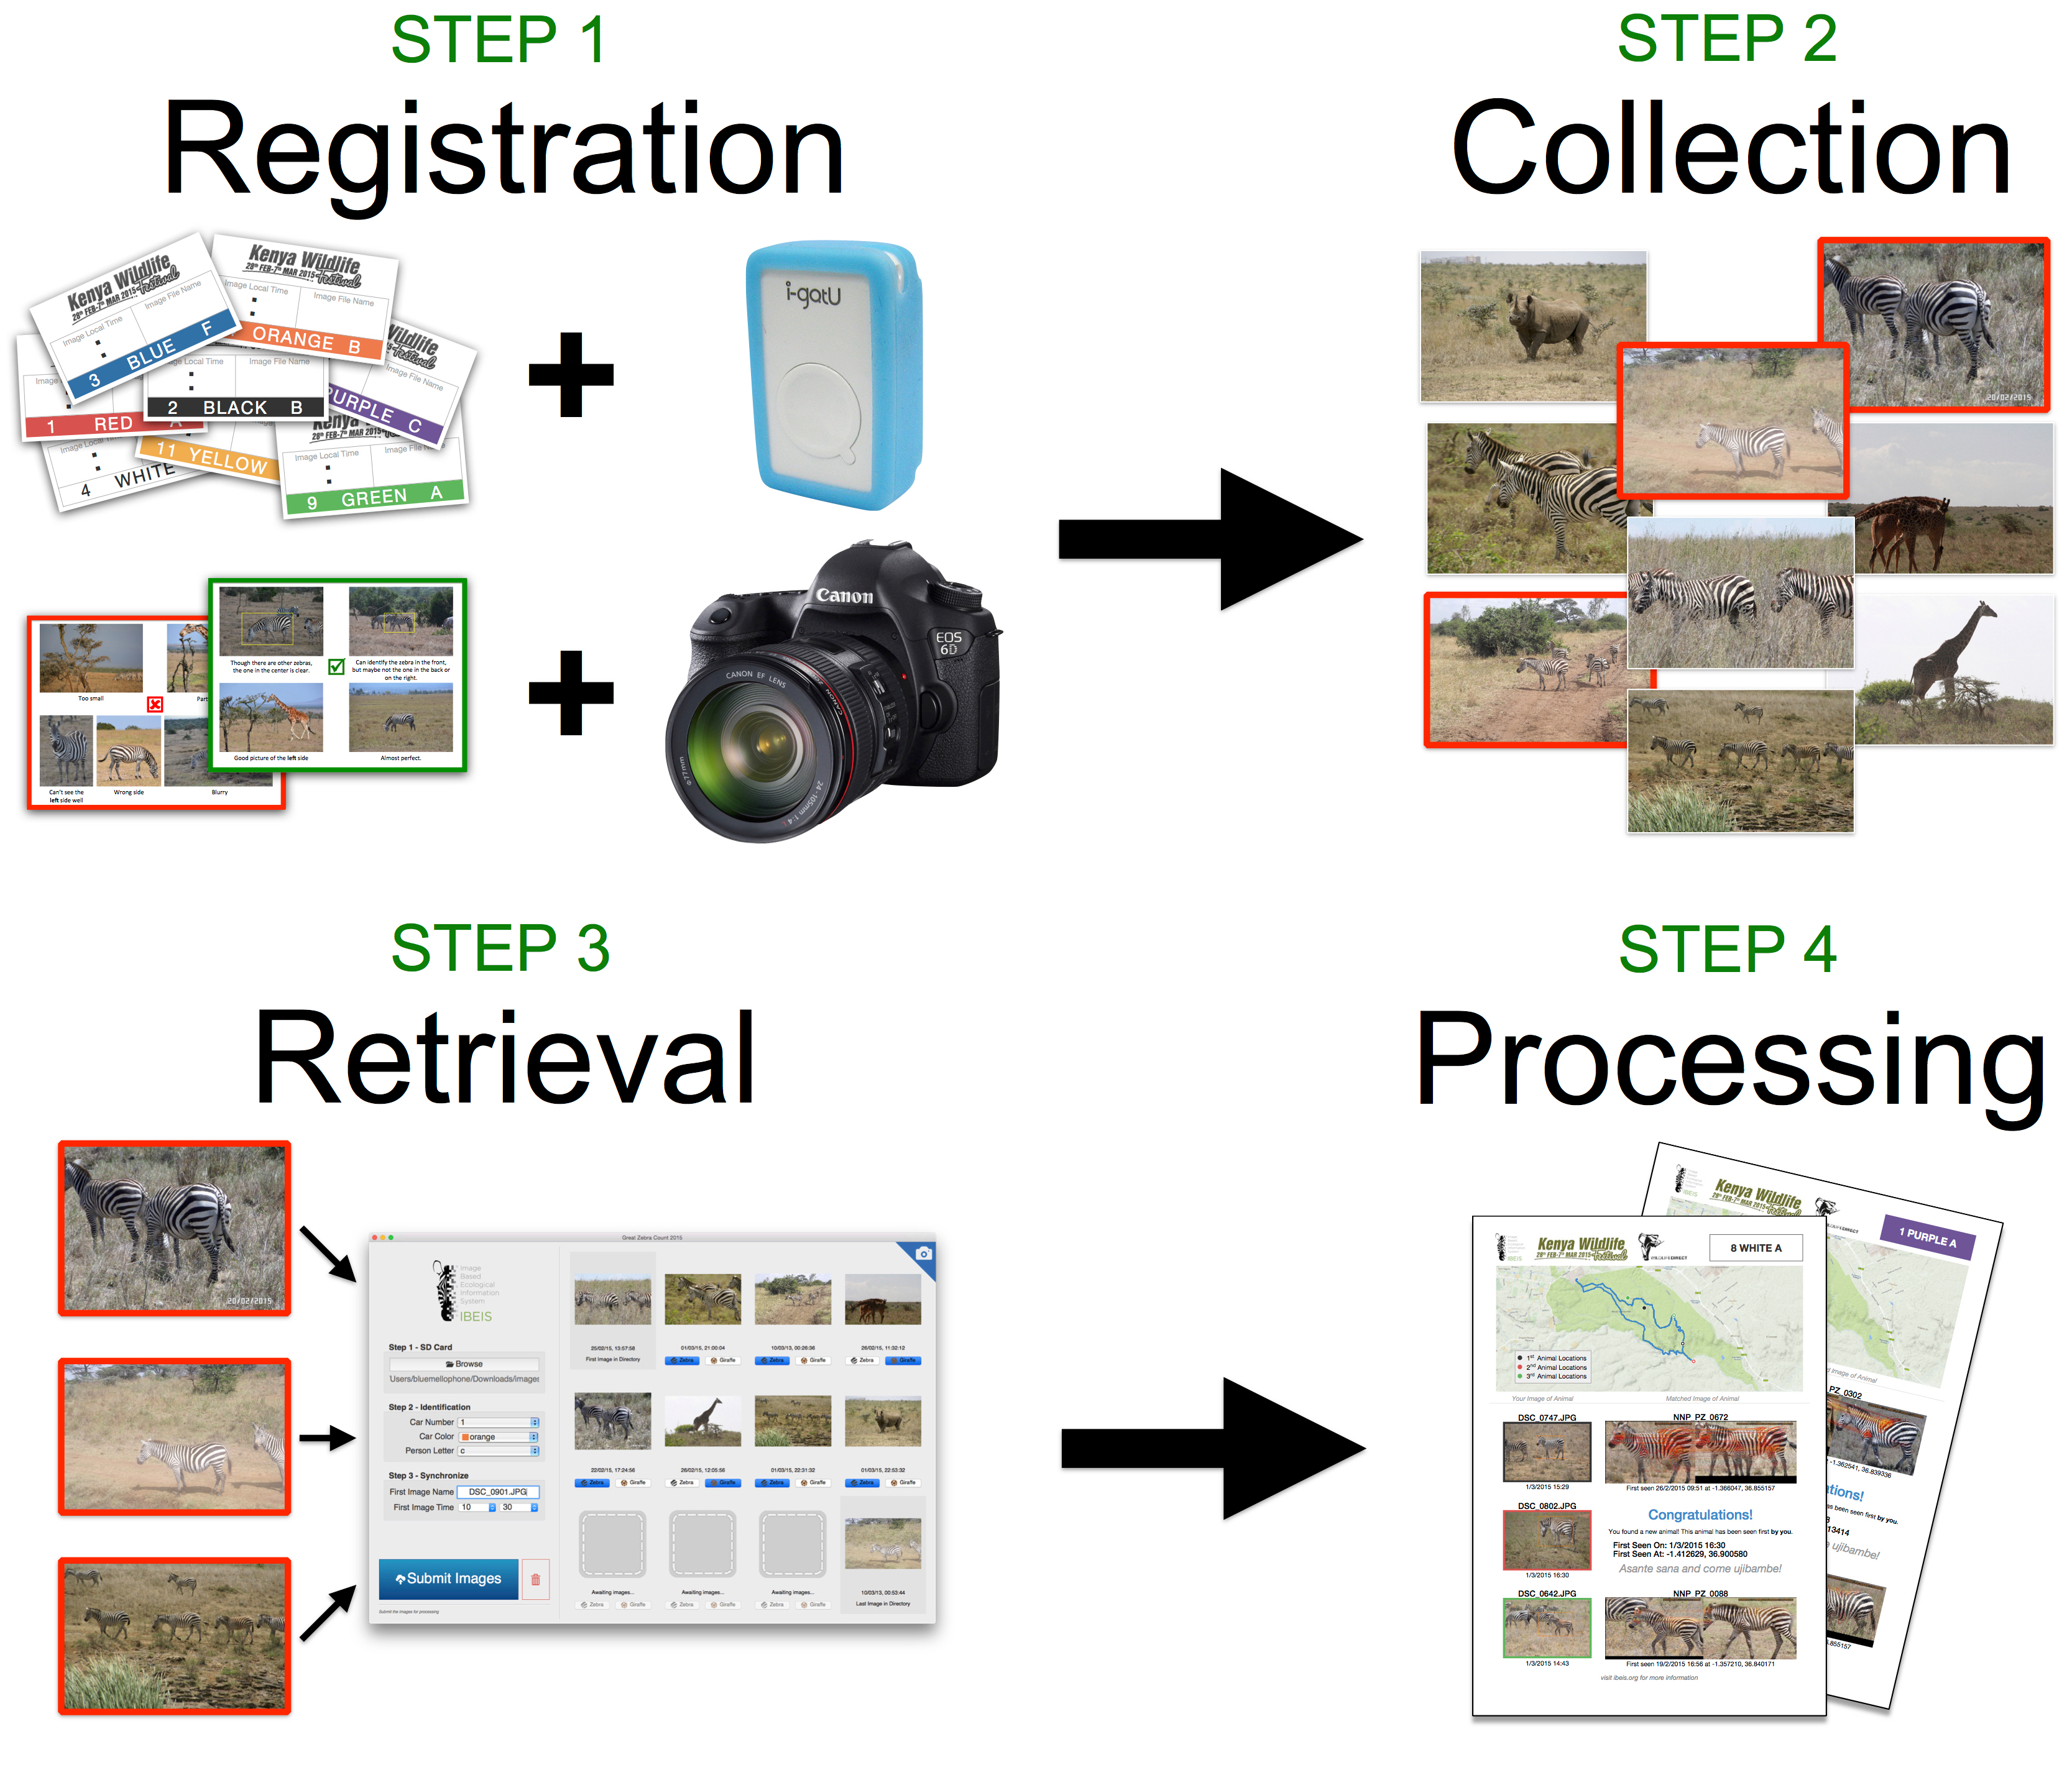
\includegraphics[width=0.90\textwidth]{resources/process_square_spaced.jpg} }}$ }}%
    \caption[Data Collection Proceedure during \textit{The Great Zebra \& Giraffe Count}]{\textbf{Data Collection Proceedure during \textit{The Great Zebra \& Giraffe Count}.}  Step 1 (Registration): citizen scientists with cameras were registered by being given a registration card, a GPS dongle (for the car), and a training sheet.  Step 2 (Collection): participants were instructed to go into the NNP and take pictures of animals for specific species and viewpoints.  Step 3 (Retieval): all images were collected from the camera of returned citizen scientists along with metadata from the registration cards and GPS dongles; a subset (in red) of the collected images were sent to IBEIS for processing.  Step 4 (Processing): the results from IBEIS were recorded into a database and tabulated onto a printout, which was given to the participant to keep as a reward for their contributions.}
        \label{fig:process}
\end{figure*}

\section{Registration}
In order to contribute images to the GZGC, each participating citizen scientist had to be given a mechanism to synchronize \textit{when} and \textit{where} their images were taken.  In order to achieve this, we trained a team of IBEIS volunteers to coordinate registration and guide participants through a time and GPS registration.  Our procedure relied on citizen scientists bringing their own personal cameras because we did not have any to lend out.  This compounded the synchronization problem as our procedure had to function across a multitude of camera manufacturers and a range of photographer experience.  In order to eliminate the complexity and inefficiencies of registration, we opted to implement a process that was agnostic to camera manufacturer, language, and specific settings and precluded the need to investigate the potential intricacies of every camera.  A team of two IBEIS volunteers guided each participant through the following registration process:

\begin{enumerate}
    \item Each photographer was given a registration card with a unique, pre-selected, identification code defined by car number, car color, and person letter. The car numbers were in the range $[0-25]$; eight colors were used (red, orange, yellow, green, blue, purple, black and white) for the car color; the person letters were in the range $[A-F]$.  Each participating car was given a number and a color combination and each person in that car was given one of the letters, for a maximum of 6 people per car. If a car had more than 6 participants (e.g.\ in the event of a school bus), additional car number and color combinations were used until there were enough registration cards to assign to each participant.  The registration card's purpose was two fold: to standardize the data collection procedure and to eventually become a memento and marketing keepsake for the participant.  The back of the registration card also had contact information for the IBEIS team and information about the software.  An example registration card for participant ``A'' in the car ``1 RED'' can be seen in Figure \ref{fig:card}.
    \item For each participant, the current, local time of registration was written on the card.
    \item Using the participant's camera, an image was taken of the participant's registration card with the then-current time.  This image -- let's call it $Image_0$ -- was required to have been taken relatively close to when the local time was written on the card (within 30 seconds), because it was used to time synchronize all images taken by that camera upon return.
    \item Once $Image_0$ had been taken, the camera's digital display was used to record the file name (or sequence number) of $Image_0$ on the registration card.  At that point, the participant was registered with the GZGC and instructed to put away and save the registration card until after data collection.
    \item Finally, each car was given an i-gotU brand GPS dongle \footnote{www.i-gotu.com/product/USB\_GPS.html [Accessed: Nov. 1, 2015]}.   The GPS dongle made a new record every second (assuming acquired satellite signal) containing the UTC timestamp, the latitude position, the longitude position, the elevation, and other metadata.  The GPS records were used to localize all of the images taken by the cameras of all participants in that car.  In the rare event that the camera provided in-camera GPS EXIF data, it was discarded and replaced by the GPS dongle's GPS record, for consistency.
\end{enumerate}
The importance of $Image_0$ cannot be overstated: it functioned as a beginning bookend for what images belonged to the GZGC and also provided a digital backup copy of the physical registration card in the event it was lost or destroyed.  Citizen scientists in the GZGC were not required to clear their camera memory cards (although encouraged) in order to participate.  During the GZGC, a citizen scientist participating with a non-empty camera memory card was the overwhelmingly dominant scenario, even though marketing material for the GZGC encouraged participants to come with a clean memory card.  For those participants, $Image_0$ was used to mark the end of potentially sensitive images, which should have not been copied from the memory card.

\begin{figure}[t]%
%\begin{figure}[!htb]%
    \centering
    \subfloat {{ $\vcenter{\hbox{ \includegraphics[width=0.45\textwidth]{resources/card-front.jpg} }}$ }}%
    \subfloat {{ $\vcenter{\hbox{ \includegraphics[width=0.45\textwidth]{resources/card-back.jpg} }}$ }}%
        \caption[The Registration Card Given to Volunteer Citizen Scientists]{\textbf{The Registration Card Given to Volunteer Citizen Scientists.}  This figure shows the front (left) and back (right) faces of an example registration card.  Each participant recieved a card with a unique identification code.  This specific card was for car ``1 RED'' and for participant ``A'' within that vehicle.  The left box of the registration card was meant to hold the time of registration and the right box to hold the image filename or sequence number of $Image_0$.}
        \label{fig:card}
\end{figure}

\section{Collection}
Once a participant was registered, they were given brief training on \textit{how} and \textit{where} to take pictures.  The assigned zones and their respective coverages of the NNP can be seen in Figure \ref{fig:coverage} in Chapter \ref{sec:results}. The training was designed to ensure sufficient image quality and to provide park coverage.  Figure \ref{fig:images} shows example images that were collected by the citizen scientists during the GZGC.

Citizen scientists were instructed to only take pictures of certain species (e.g.\  zebra) and of consistent viewpoints (e.g.\ left-side).  We did not have to teach the differences between sub-species of zebra or giraffes considering the NNP only had the one sub-species of each, plains zebra (\textit{Equus quagga}) and Masai giraffe (\textit{Giraffa camelopardalis tippelskirchi}).  The viewpoint constraint resolves a symmetry ambiguity, which is caused by zebras (and giraffes) not being left-right symmetric (i.e.\ the left-side appearance is different from the right-side).  Therefore, due to this lack of symmetry, we cannot reliably know if we have seen an individual before if we only saw opposite sides.  Lastly, the participants were asked to avoid taking obstructed, poorly illuminated, or out-of-focus pictures or where the zebra was too distant to get a detailed picture.

To ensure park coverage, each participating car was assigned a zone within the NNP to take pictures.  Participants were instructed to start taking pictures only from inside their assigned zone, but they could continue to take pictures outside of their zone as they returned back to the registration site.  This constraint was to ensure adequate coverage of the assigned zone by attempting to reduce ``species fatigue'' -- the phenomenon where a photographer tires of taking pictures of a common species -- since it produces a sampling bias in the locations of animal sightings.  This bias can be tolerated outside of a participant's assigned zone, but should be discouraged in order to achieve a higher likelihood of capturing unbiased animal sightings in all zones.

\begin{figure*}[t]%
    \centering
    \subfloat {{ $\vcenter{\hbox{ 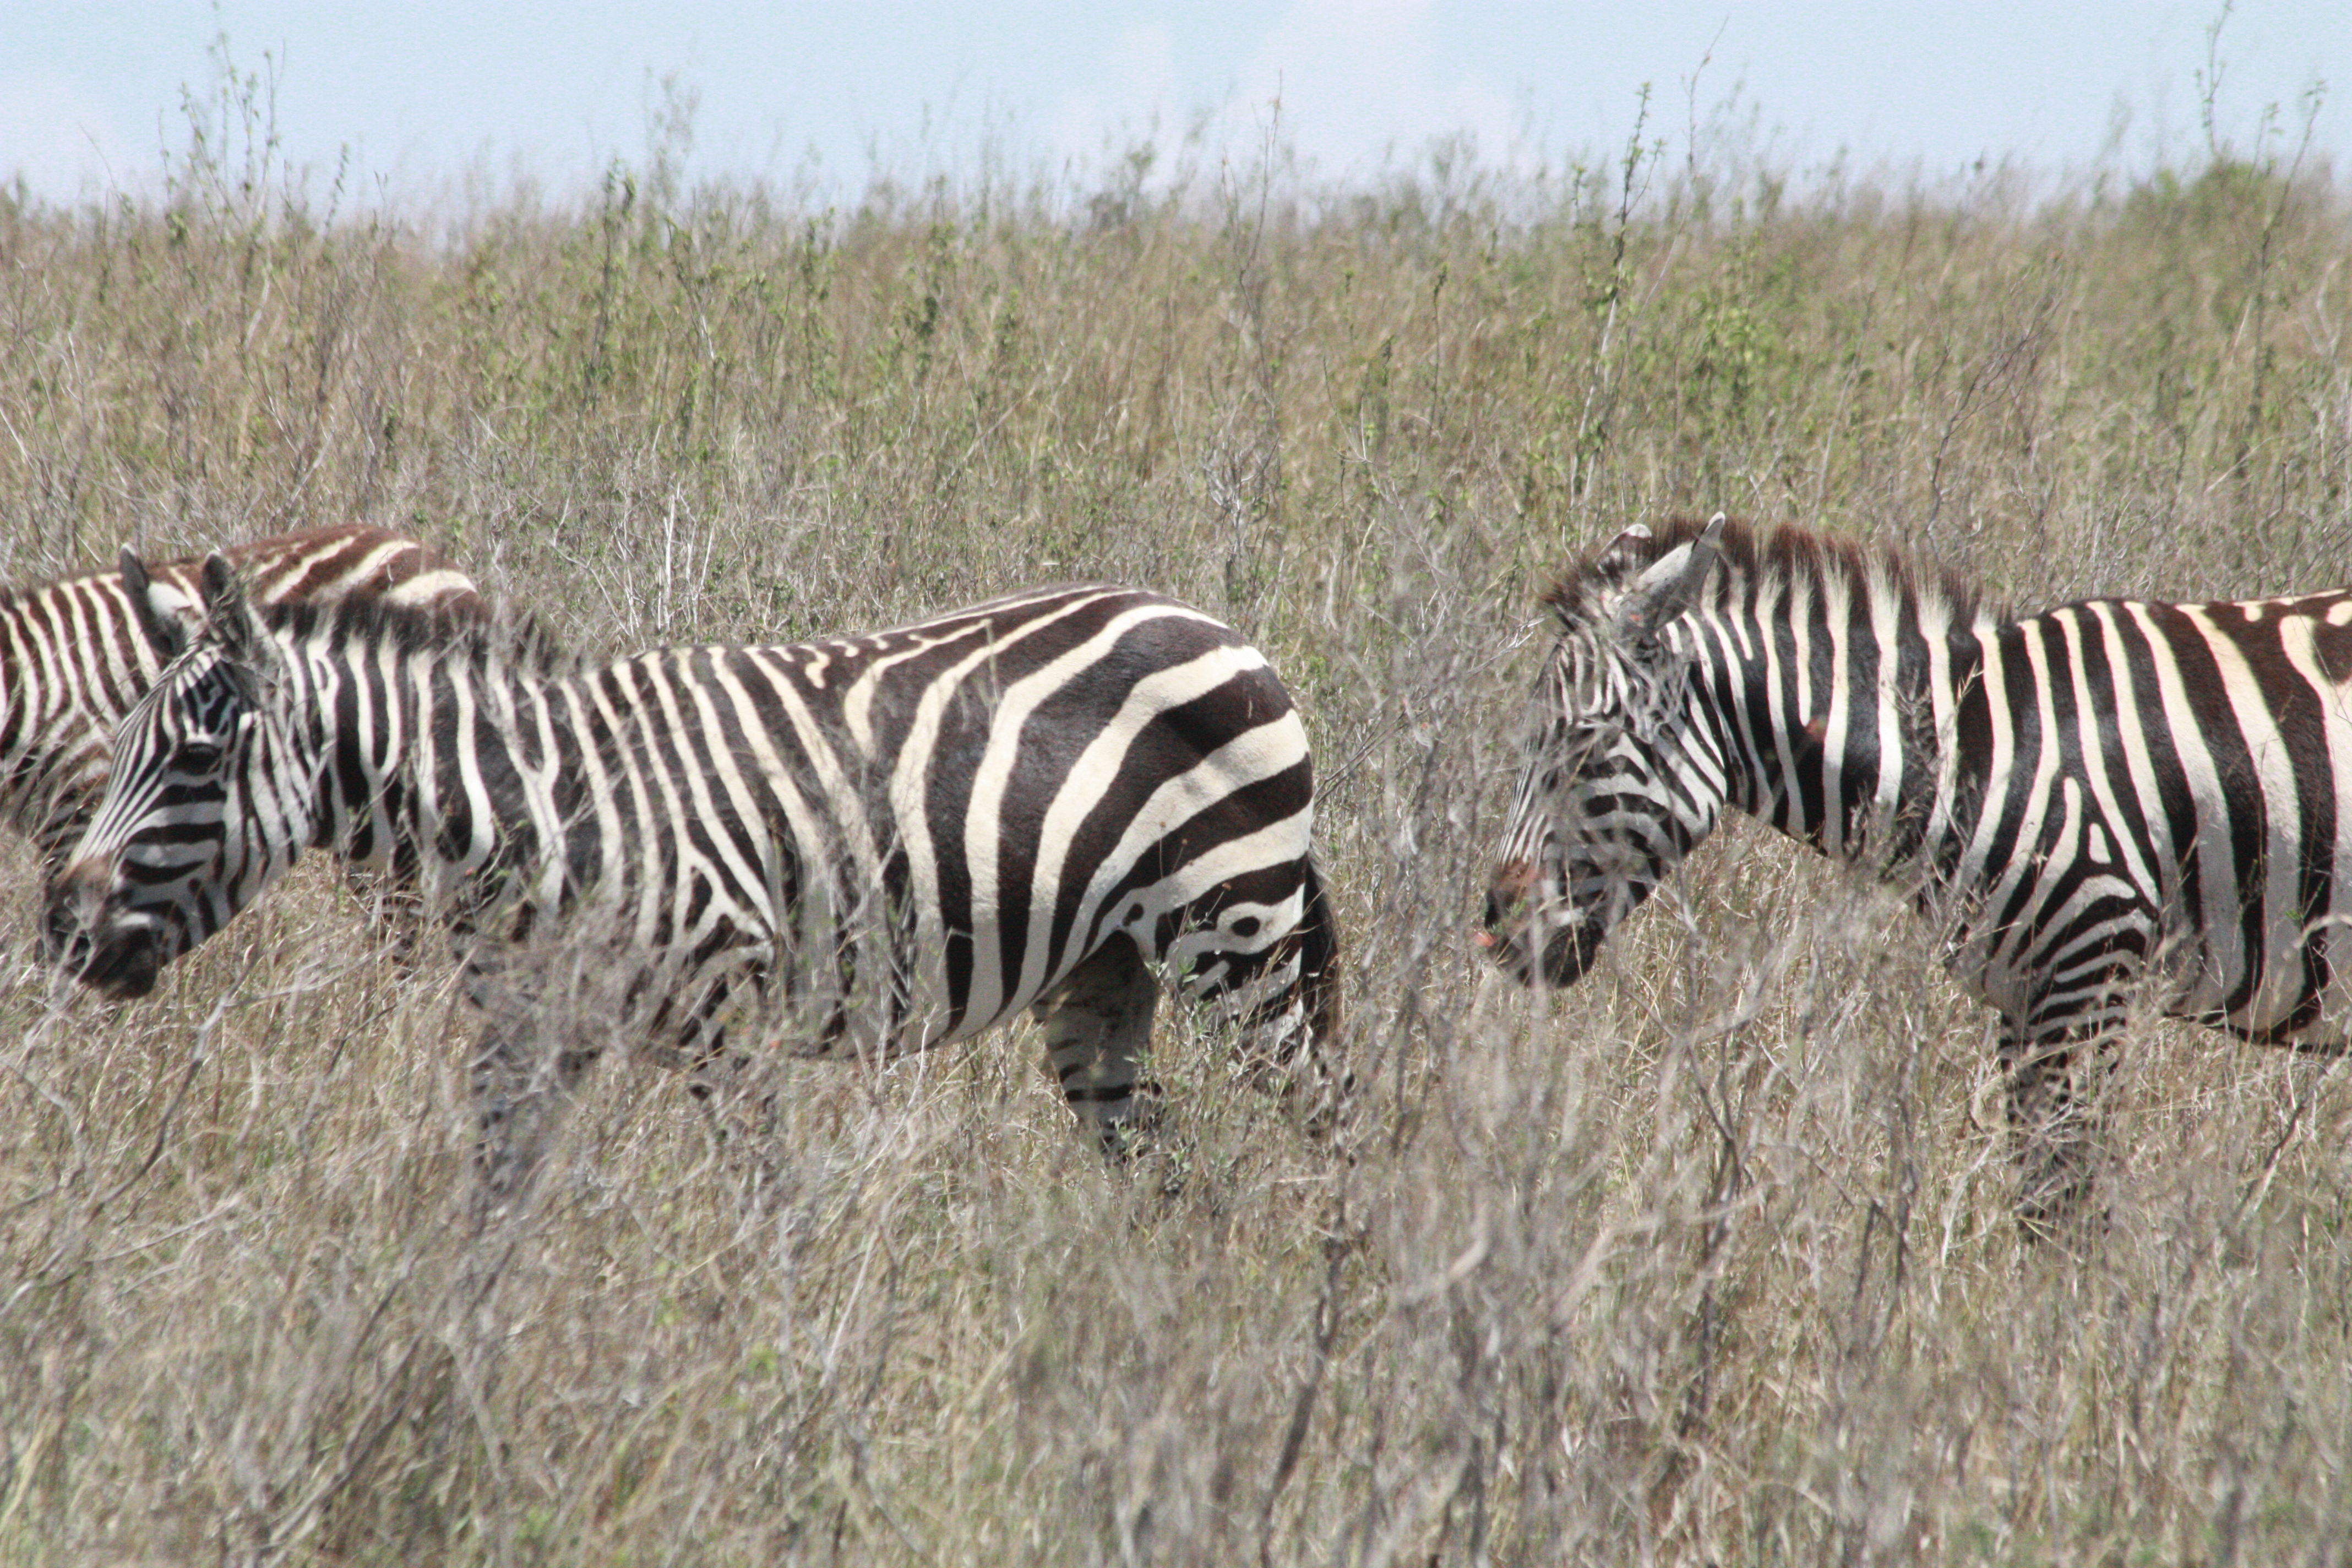
\includegraphics[width=0.16\textwidth]{resources/images/0b236c57-5023-e3e1-8c5d-c5a55d346ea8.jpg} }}$ }}%
    \subfloat {{ $\vcenter{\hbox{ \includegraphics[width=0.16\textwidth]{resources/images/0b456b34-dc14-3d3f-3dfa-833a3a31c8d1.jpg} }}$ }}%
    \subfloat {{ $\vcenter{\hbox{ 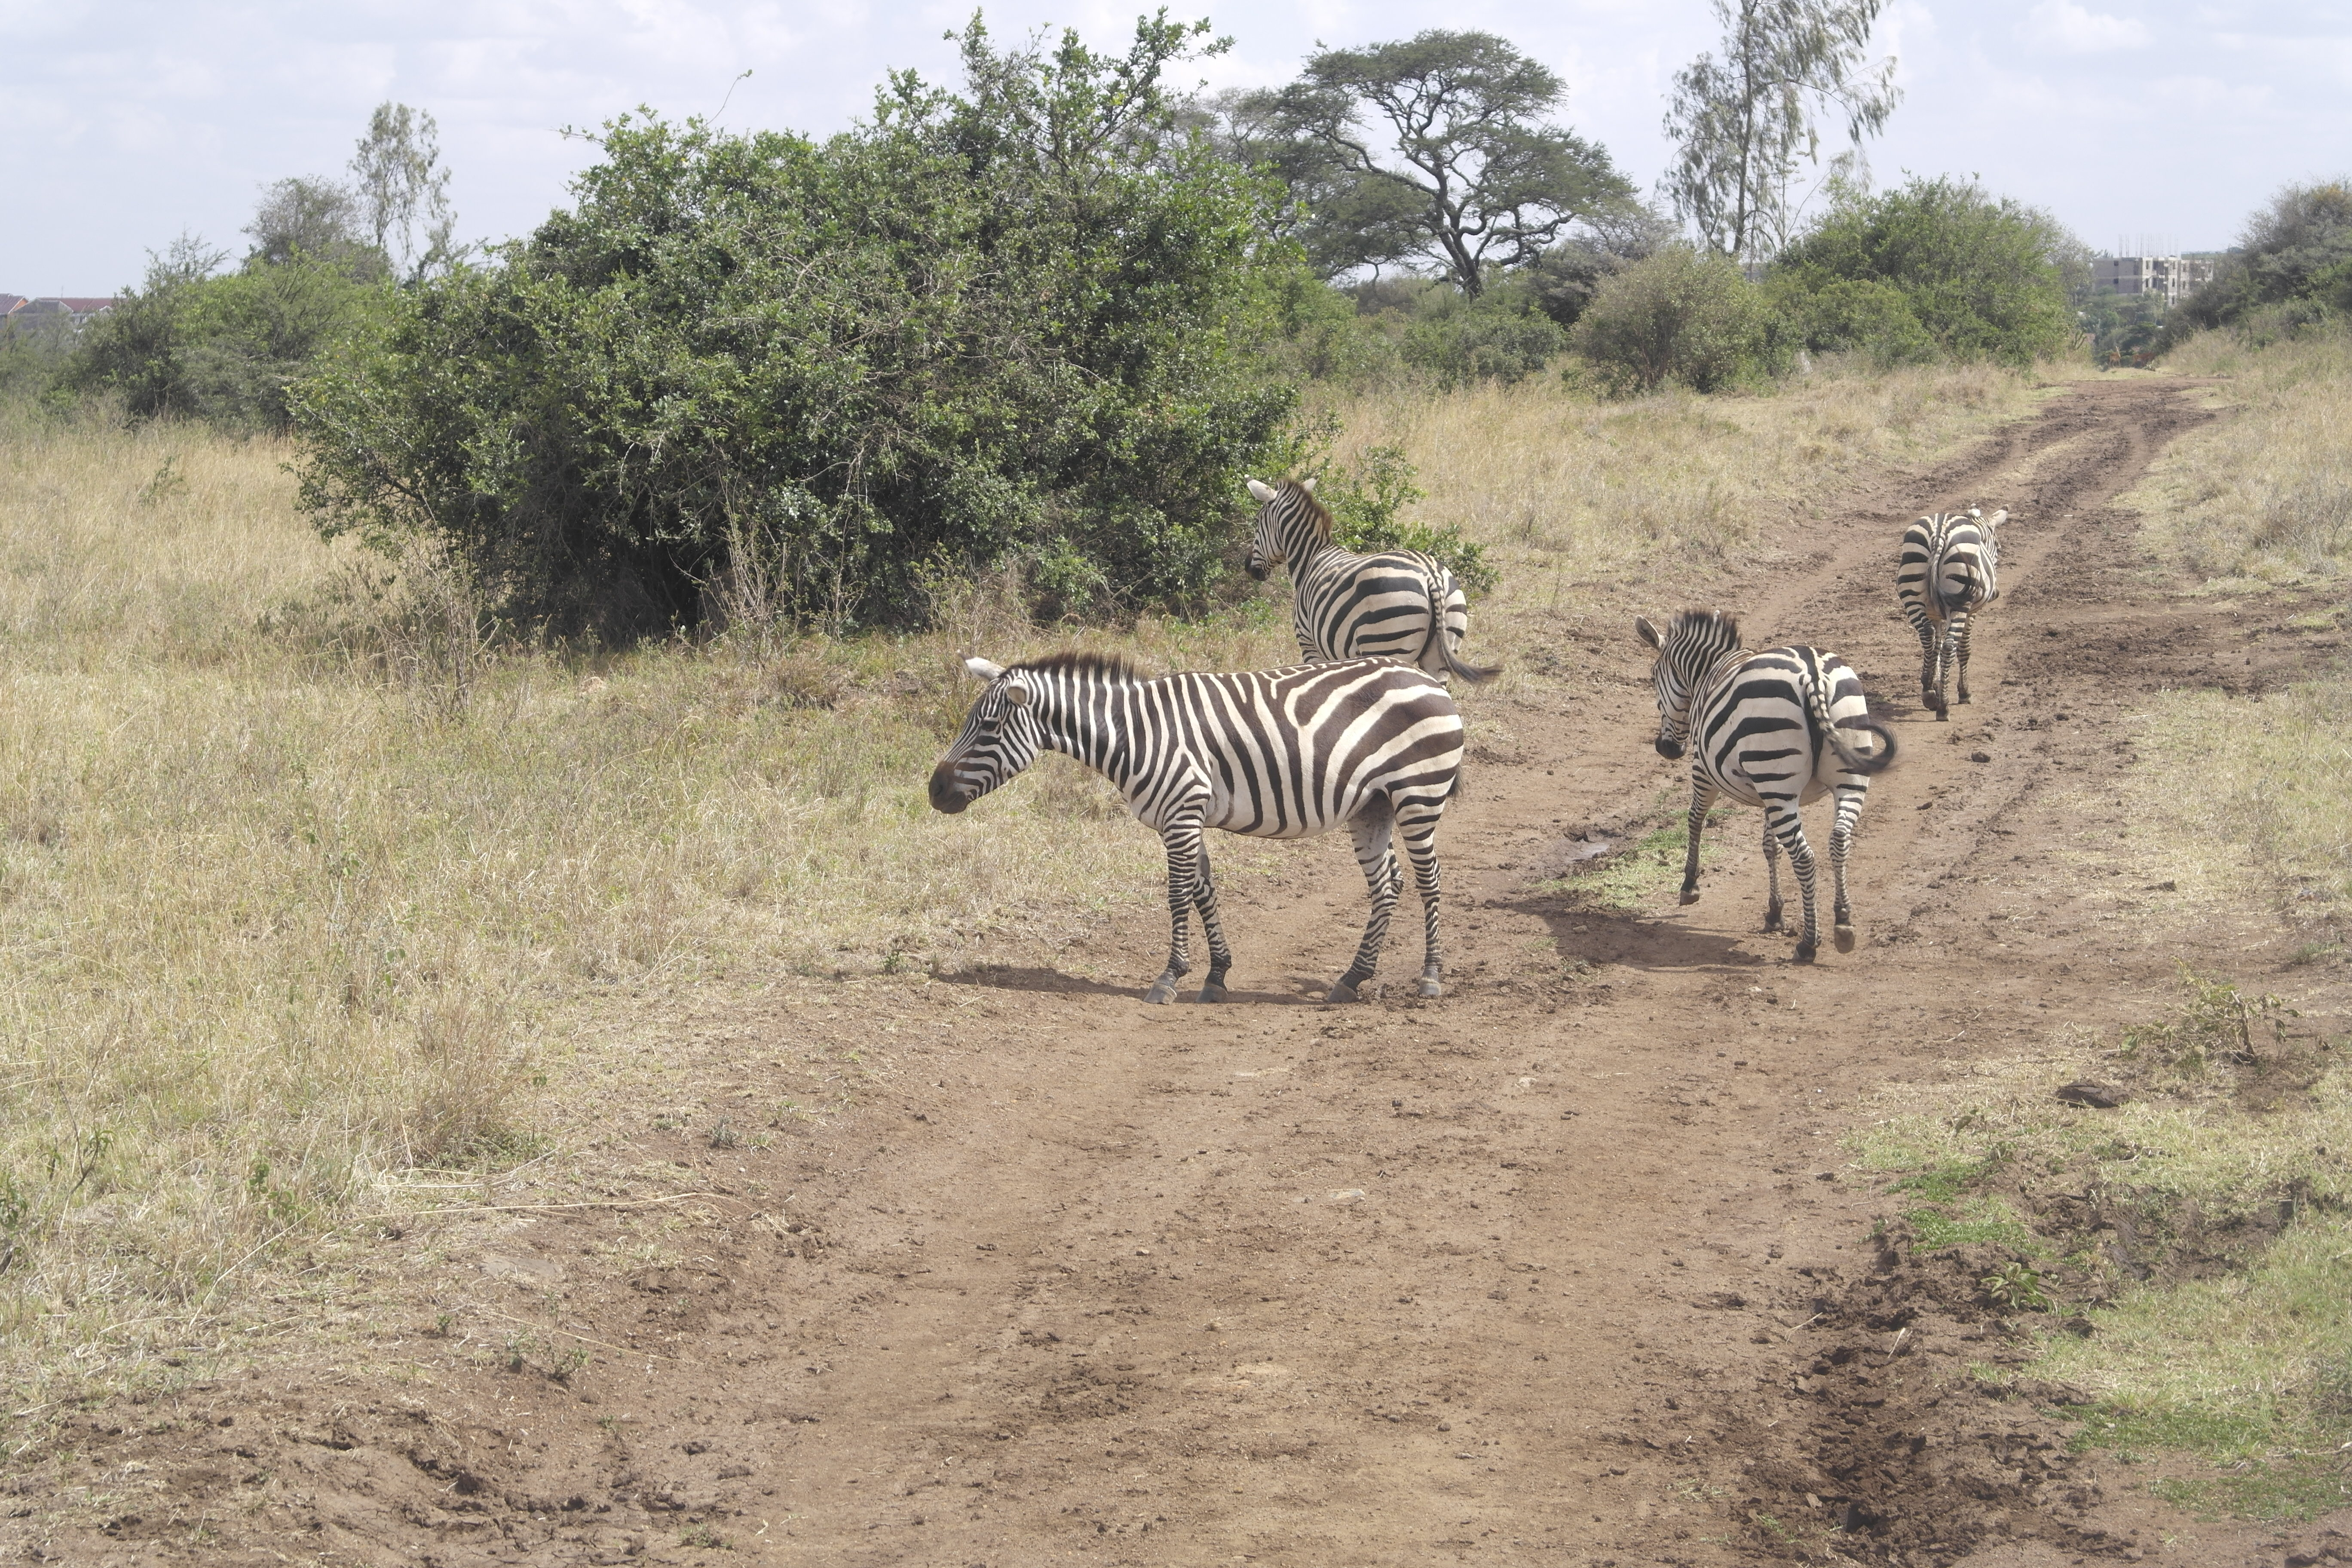
\includegraphics[width=0.16\textwidth]{resources/images/0b6993d5-ee88-04b3-0953-8a508857da42.jpg} }}$ }}%
    \subfloat {{ $\vcenter{\hbox{ 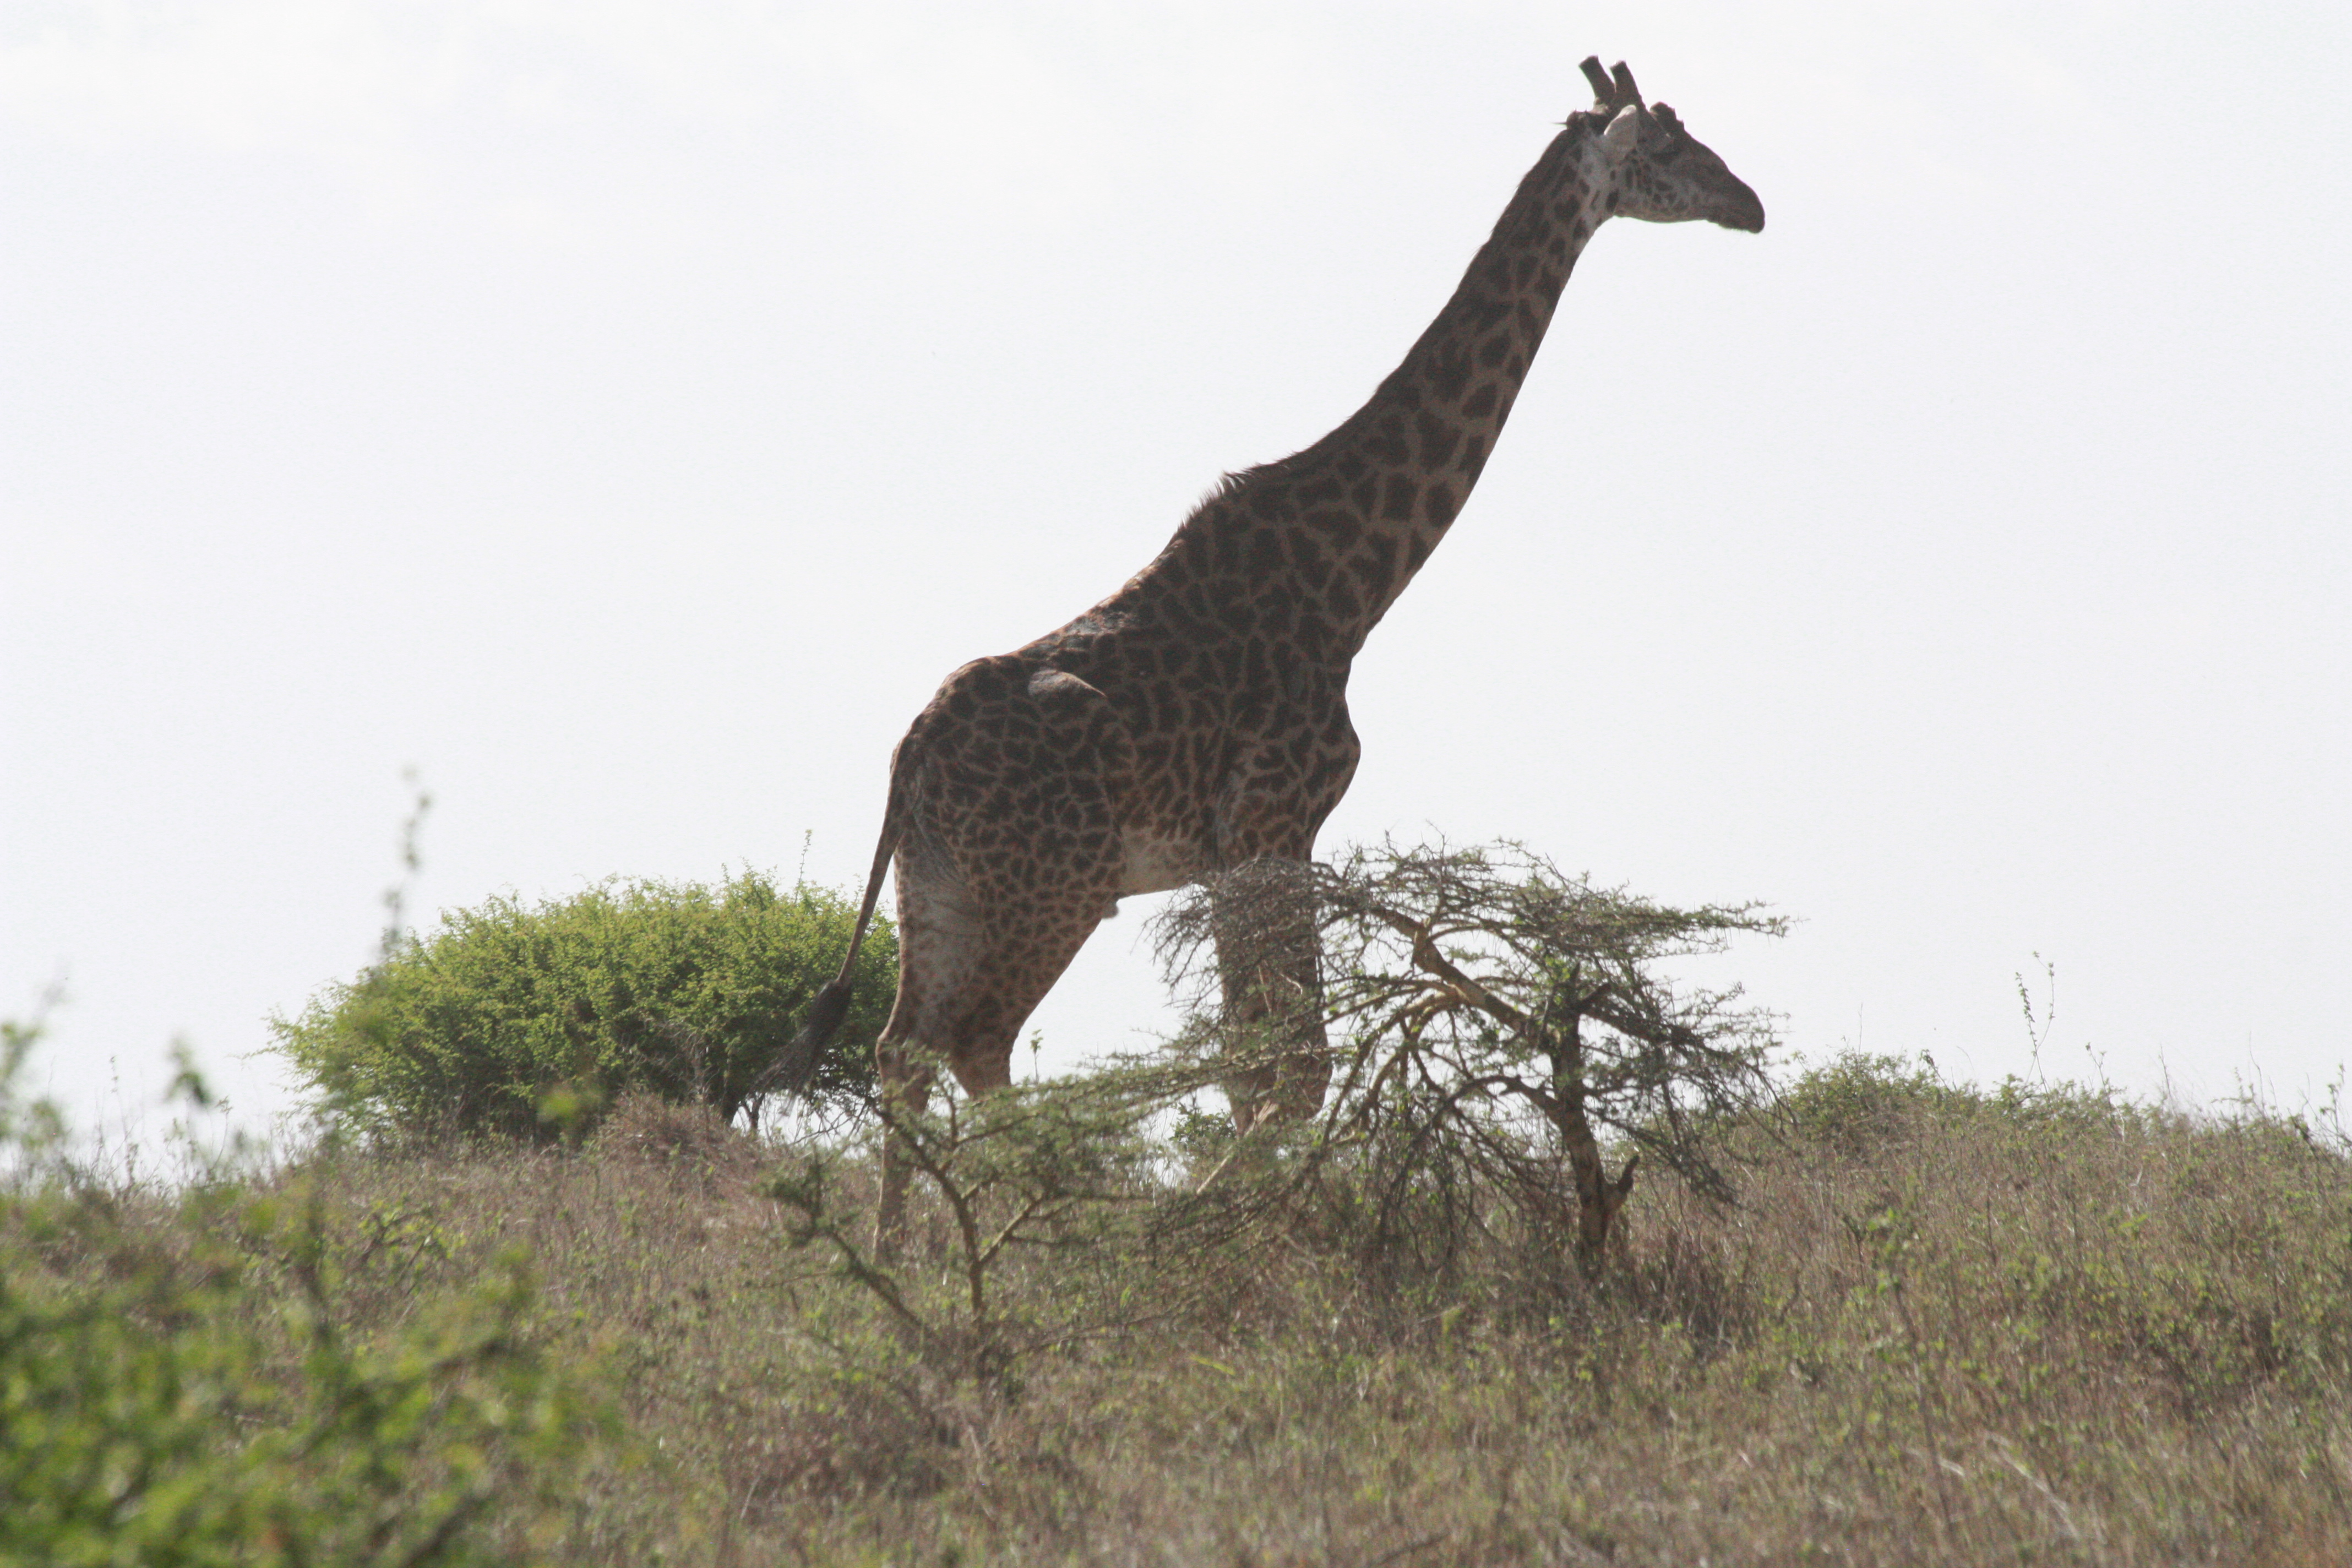
\includegraphics[width=0.16\textwidth]{resources/images/0c81eb06-0c4f-beba-cddb-858d59db523d.jpg} }}$ }}%
    \subfloat {{ $\vcenter{\hbox{ 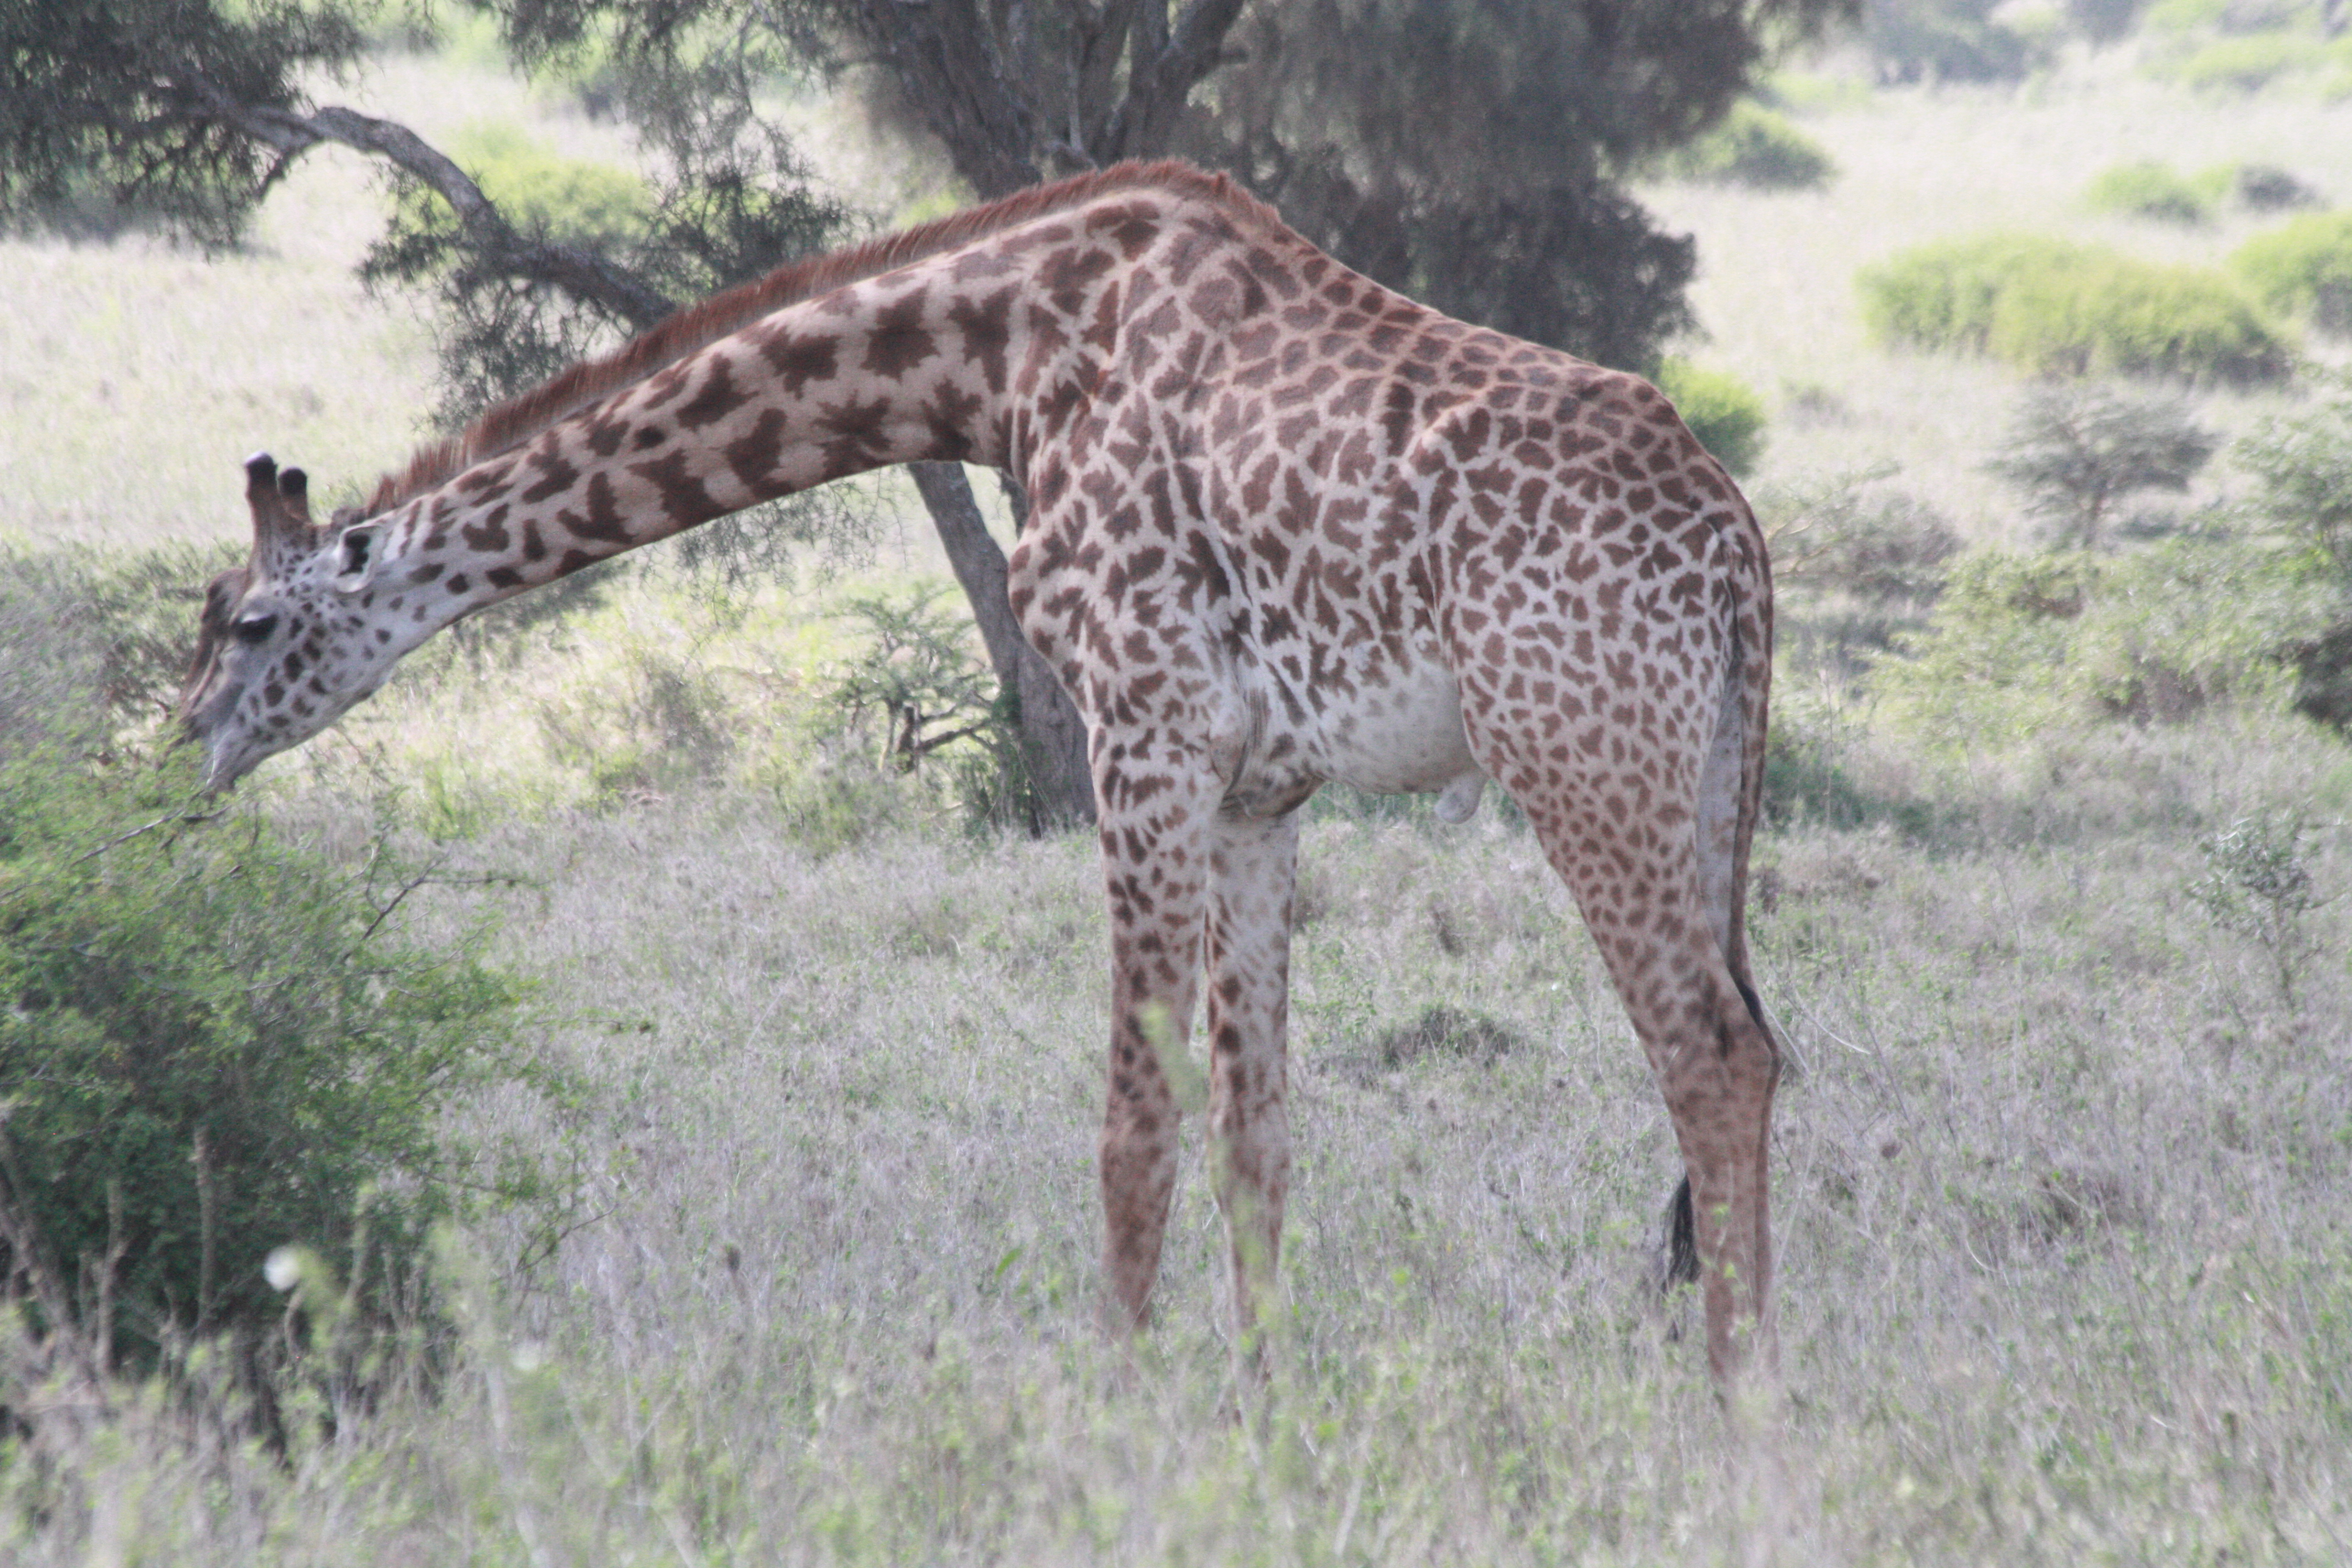
\includegraphics[width=0.16\textwidth]{resources/images/3d71a3d7-fef9-cfb4-0f28-c170338705f0.jpg} }}$ }}%
    \vspace{0.1cm}
    \subfloat {{ $\vcenter{\hbox{ 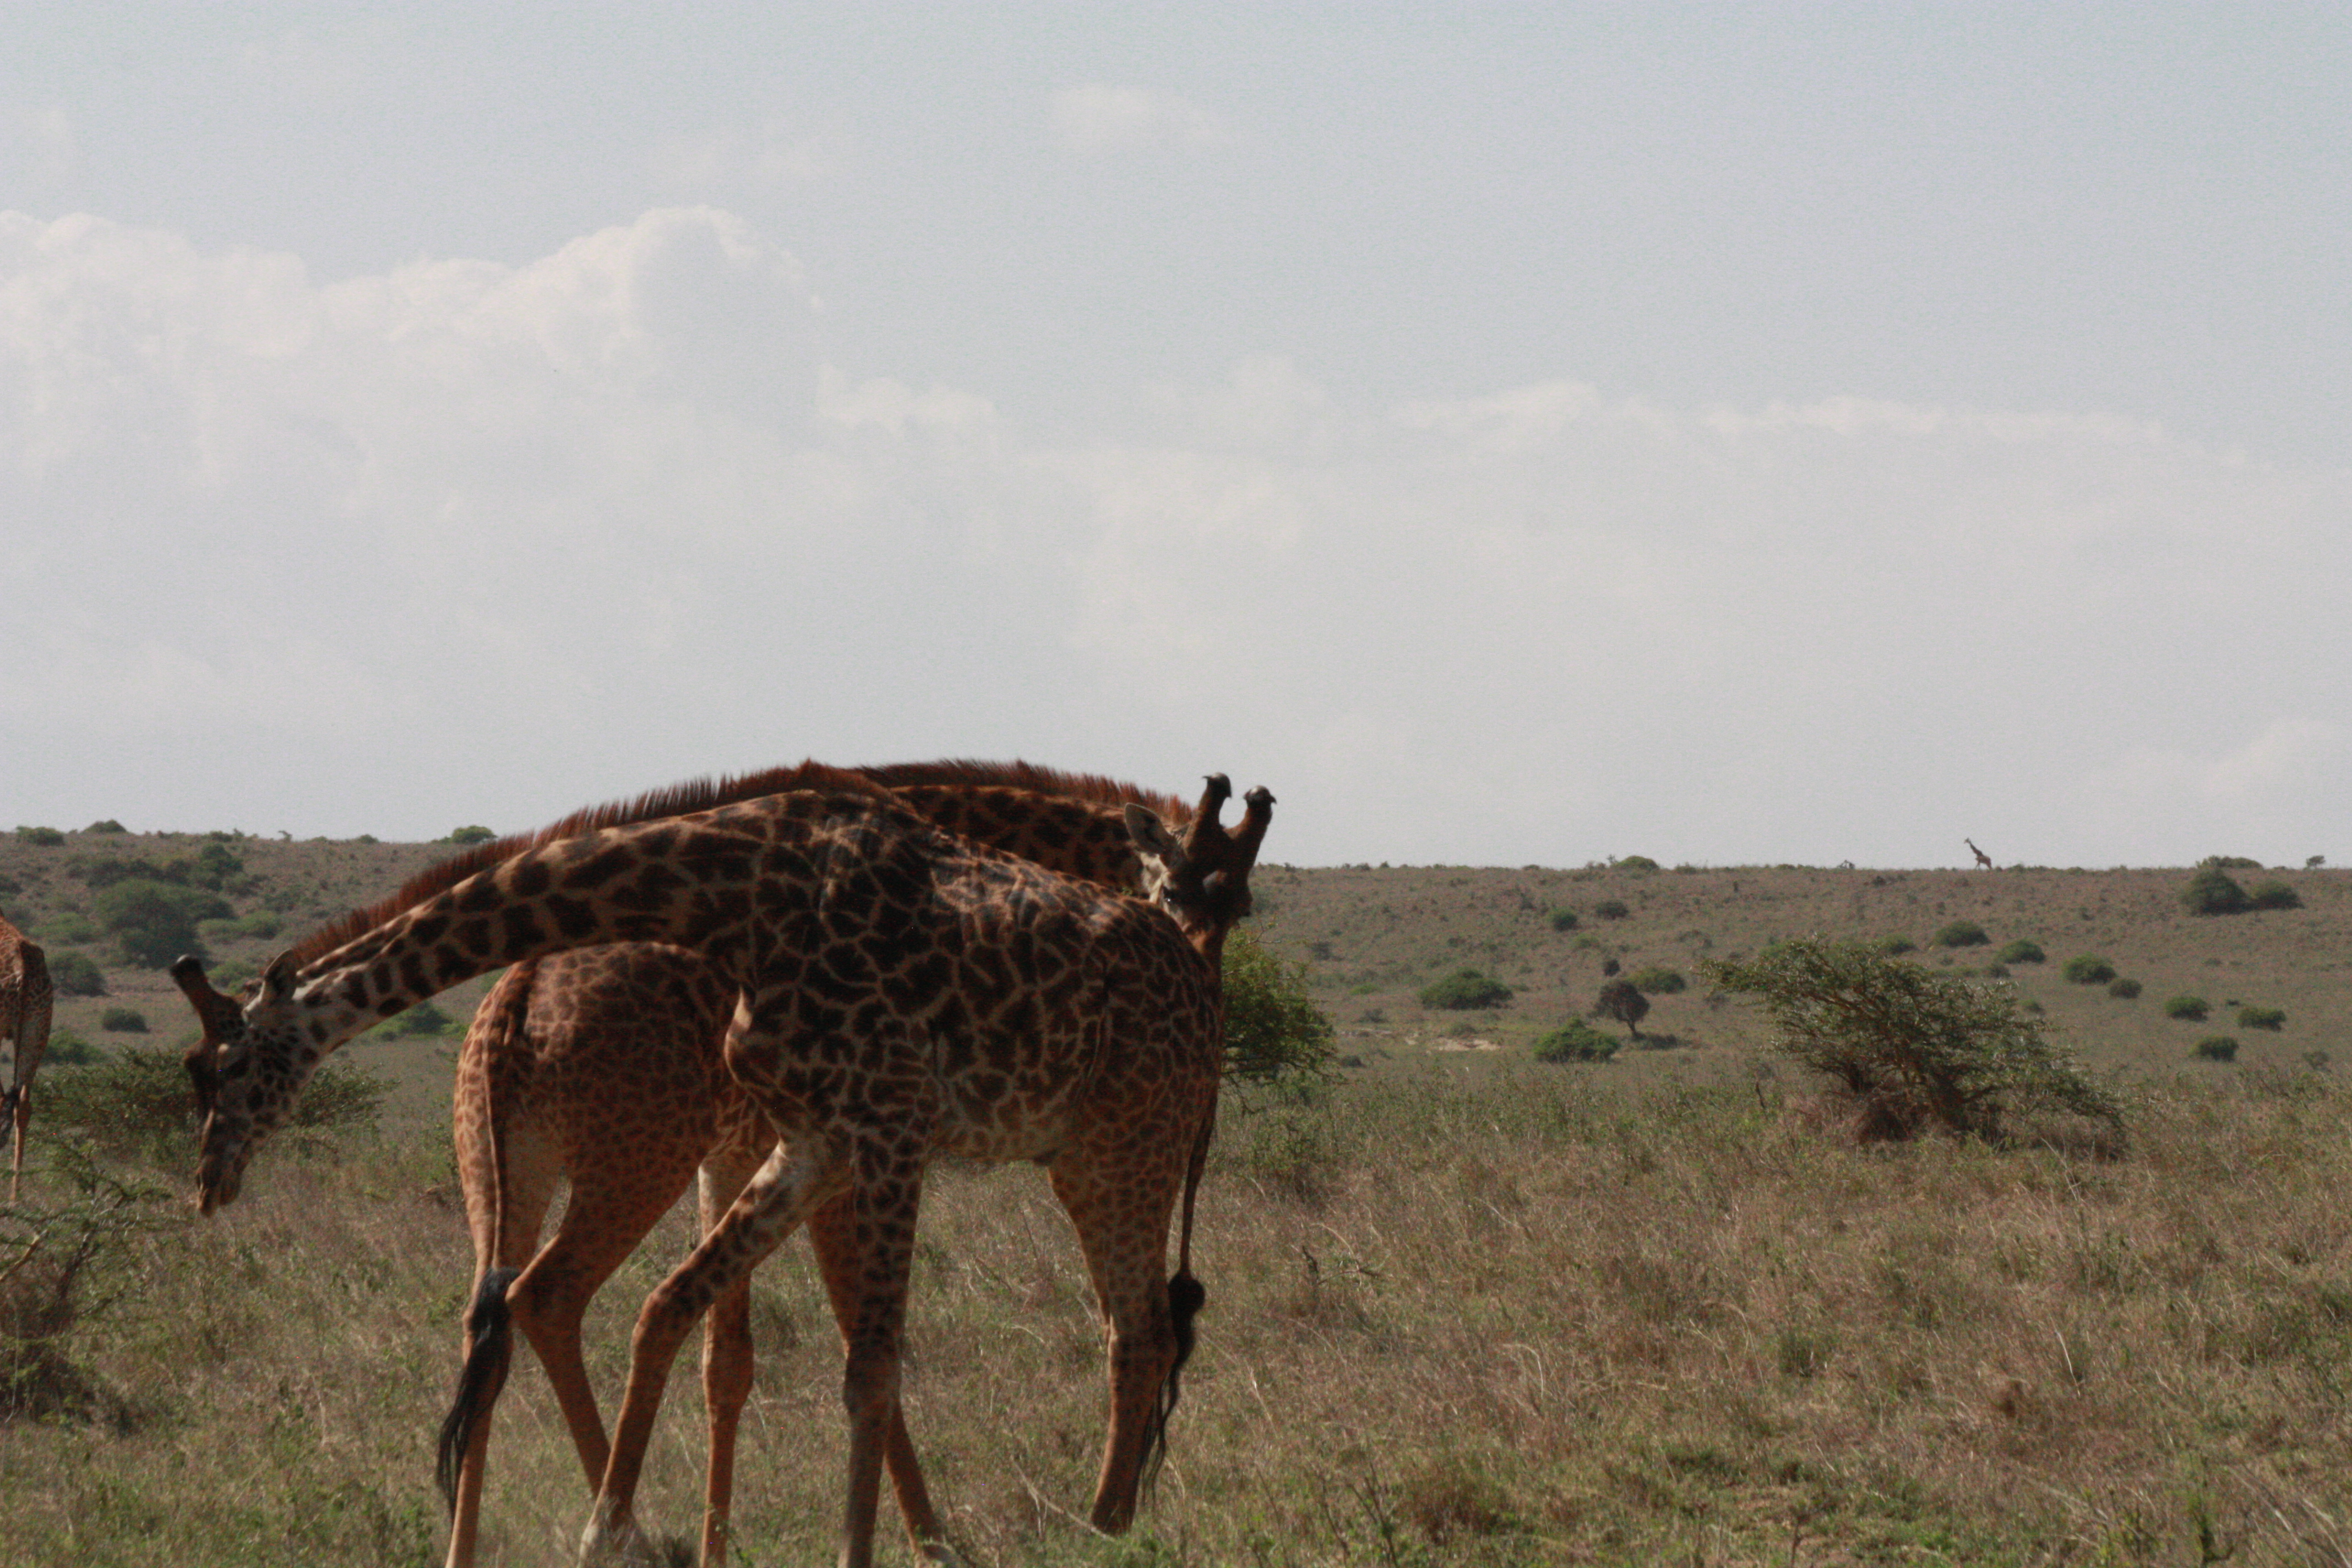
\includegraphics[width=0.16\textwidth]{resources/images/0c166bc9-7e21-6837-f09f-976a96f28f28.jpg} }}$ }}%
    \subfloat {{ $\vcenter{\hbox{ \includegraphics[width=0.16\textwidth]{resources/images/0c381b04-1651-4a1c-a24f-fe975a5f648d.jpg} }}$ }}%
    \subfloat {{ $\vcenter{\hbox{ \includegraphics[width=0.16\textwidth]{resources/images/0cf36e40-07f7-8003-adae-544b8416f4a0.jpg} }}$ }}%
    \subfloat {{ $\vcenter{\hbox{ \includegraphics[width=0.16\textwidth]{resources/images/0d0f8f63-3853-ae0f-409e-5ed351339045.jpg} }}$ }}%
    \subfloat {{ $\vcenter{\hbox{ 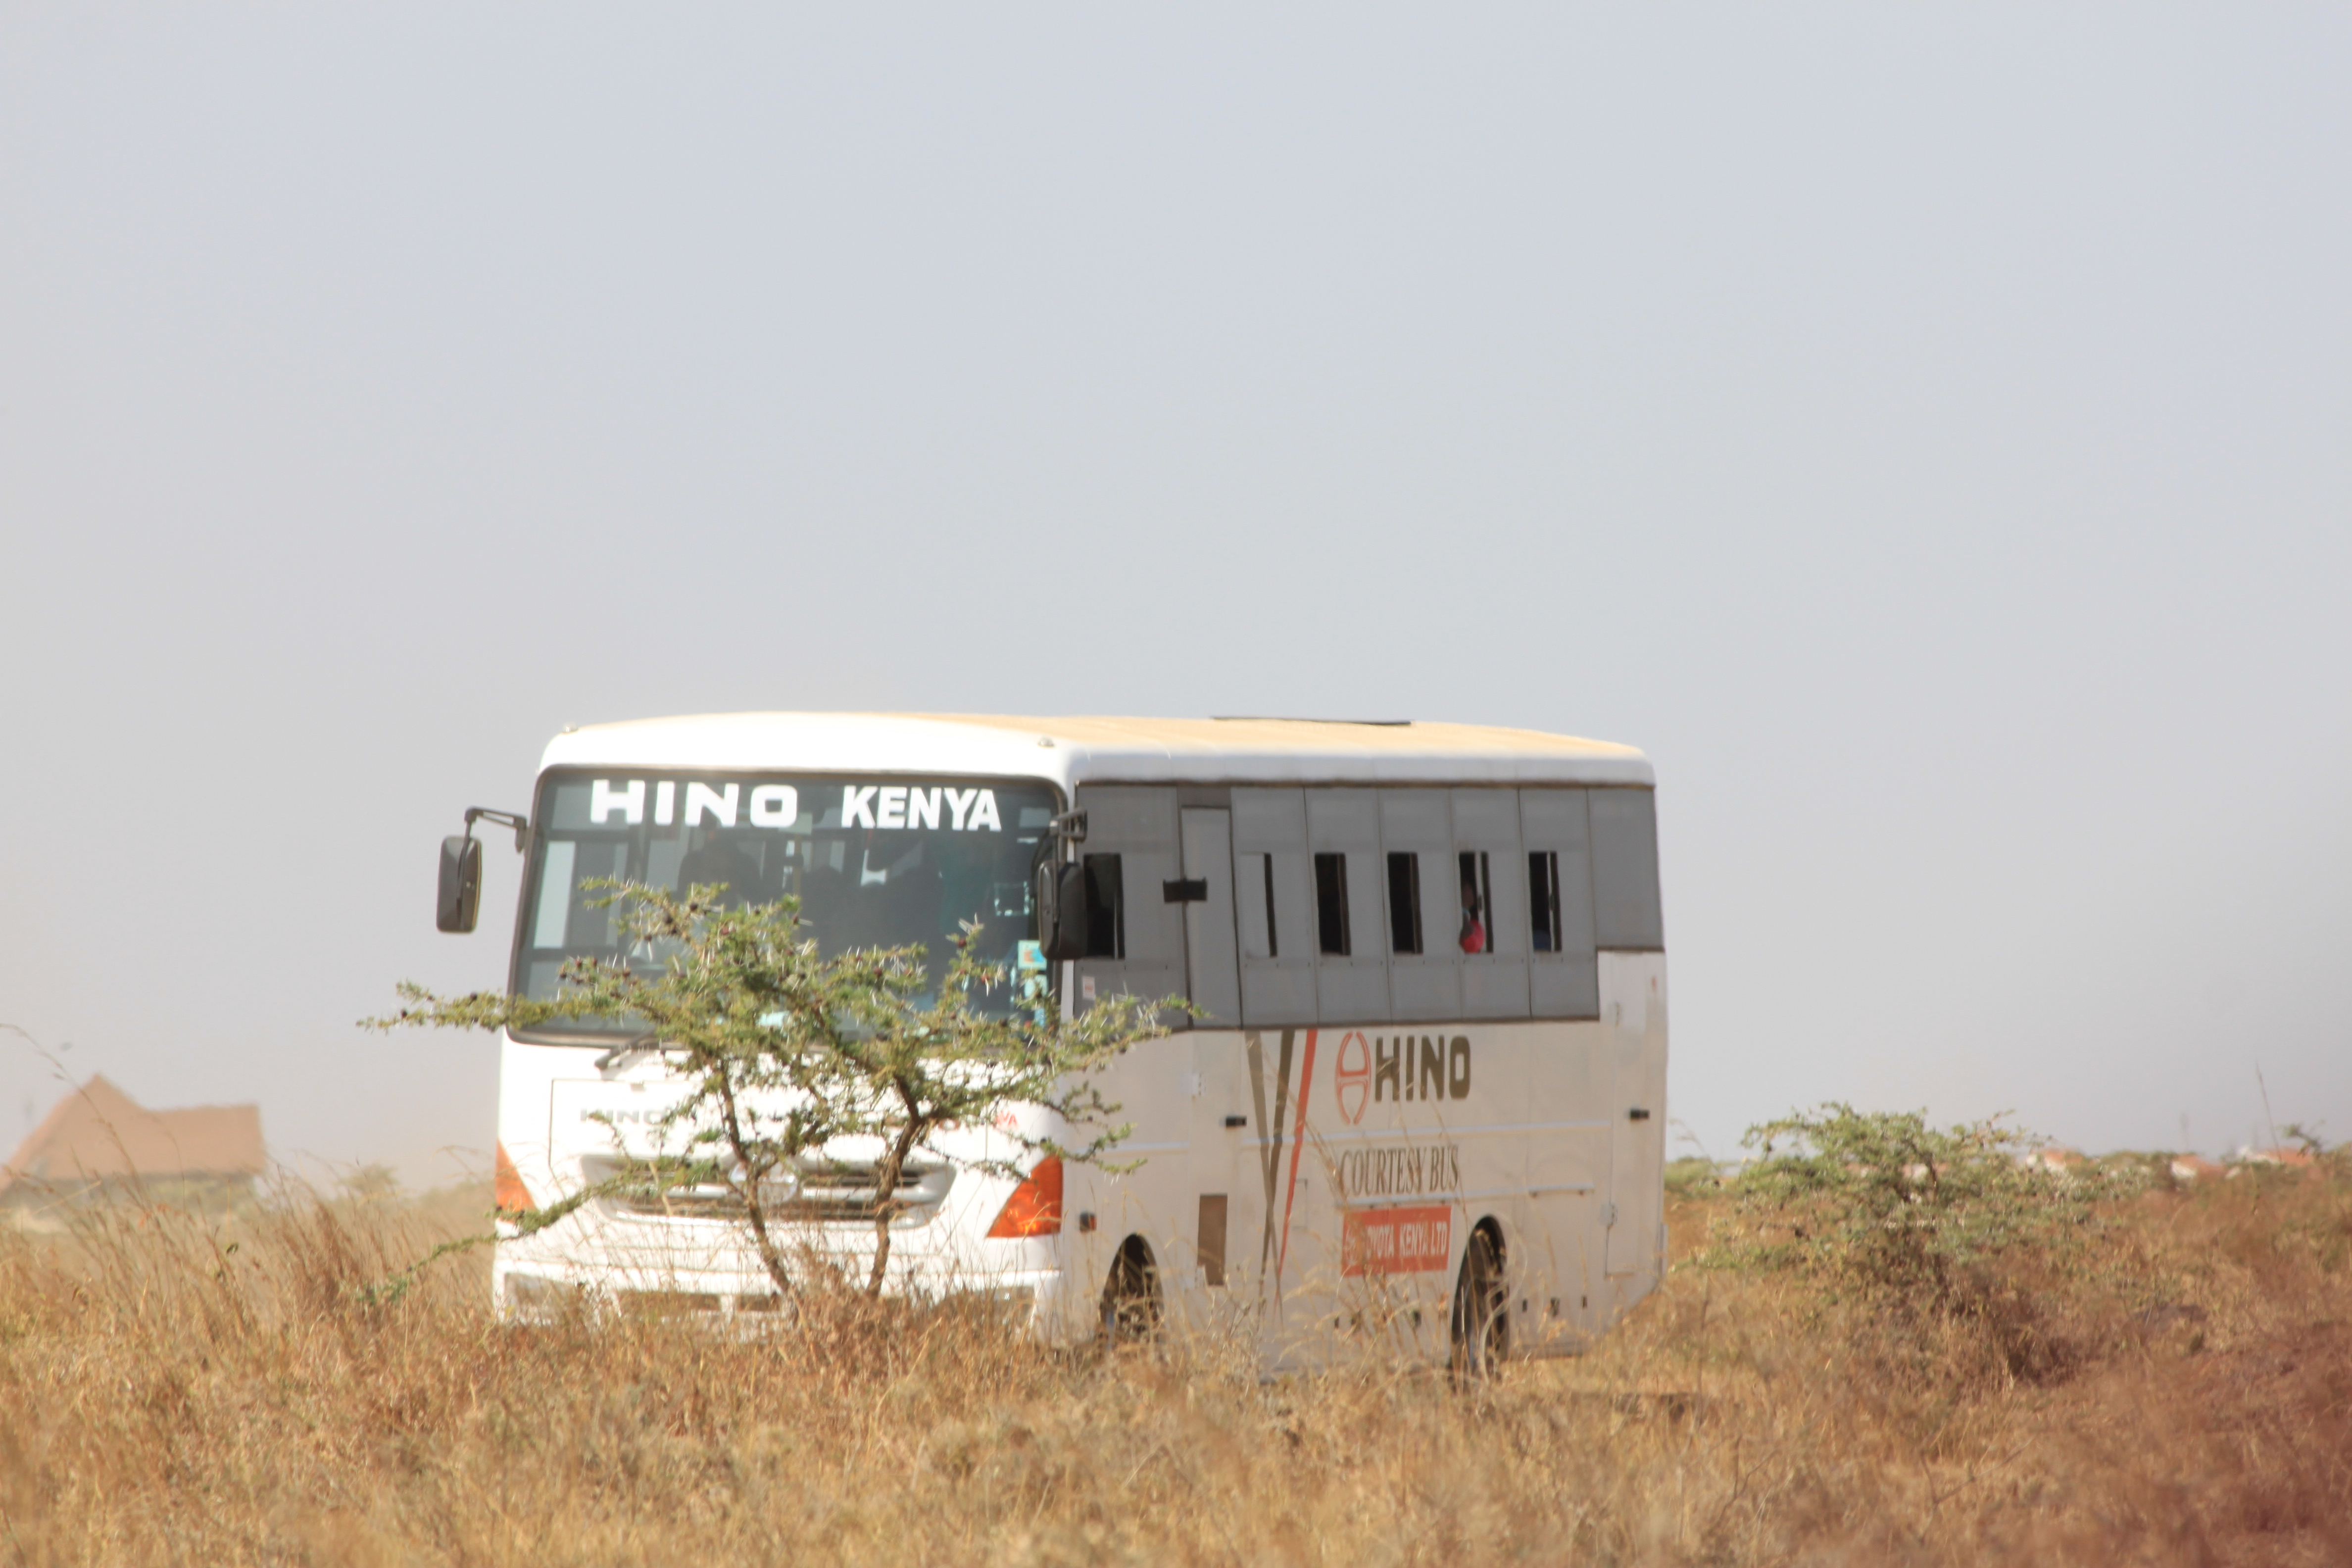
\includegraphics[width=0.16\textwidth]{resources/images/0e507f8d-b13c-b49d-fd19-f00d9570dbd7.jpg} }}$ }}%
    \vspace{0.1cm}
    \caption[Example Images Collected during \textit{The Great Zebra \& Giraffe Count}]{\textbf{Example Images Collected during \textit{The Great Zebra \& Giraffe Count}.}  A set of 10 example images collected from citizen scientists in the Nairobi National Park.  Images were collected from a variety of camera types, image formats, and across many hours throughout the day.  Most images contain sightings of zebra, giraffe, elephant, rhinocereous, cars, or birds from a wide range of focus, zoom, lighting conditions, and viewpoints of the animals.  There were also negative images collected having no animals in the forground, but instead had only road, cars, people, man-made structures, and planes, as shown in the bottom right image.  A total of 9,406 images were collected from all citizen scientists; a detailed breakdown of all images contributed can be found in Figure \ref{fig:contributions}.}
        \label{fig:images}
\end{figure*}

\section{Retrieval (Client)} \label{sec:retrieval}
Once the data collection was complete for a particular car, the participants were instructed to return to the registration site to contribute their images to the GZGC.

A participant's camera was required to have some form of removable memory card so that the images could be retrieved easily.  As such, mobile devices and camera phones were not recommended (but not explicitly excluded) for the sake of an efficient data collection workflow.  Fortunately for the GZGC, this was not considered much of a limitation considering most current mobile devices and camera phones do not have sufficient optical capabilities for capturing usable images.   Notably, the lack of a zooming lens and a limited optical sensor degrade the usefulness and quality of the images.  When no other camera was available to a participant, mobile devices and camera phones were permitted on the condition that the images could still be retrieved from a memory card or retrieval did not rely on dedicated or proprietary extraction software.  For the GZGC, we only had two contributors who took pictures using a mobile device.  The images contributed by these citizen scientists were not of optimal quality and IBEIS had trouble identifying correct matches due to lens artifacts and the photographed animals being too small in the image.

For other data collection events, a mobile data collection device might be tolerable (or even preferred) and a more sophisticated workflow or mobile application (app) could be created to facilitate offloading the image data from the device.  An app could be downloaded to the phone and used to collect and annotate using a light-weight, touch-based user interface.  The app could also implement a communication protocol that would allow sending the collected images directly to a central server for processing, without the need to download the images to a client machine.

Using the registration card, the participant's camera memory card, and the car's GPS dongle, all of the information required for processing could be gathered:

\begin{enumerate}
    \item Using the participant's physical registration card, the participant's identification code and the file name (or sequence number) for $Image_0$ could be recovered.
    \item Images were copied, in order of the EXIF timestamp provided by the camera, from the memory card starting at $Image_0$.  All images were copied locally to the import client laptop and a copy was saved onto an attached backup external hard-drive.
    \item The registration card also provided when $Image_0$ was taken in Nairobi local time.  Therefore, assuming the camera was properly keeping time and the EXIF timestamps were self-consistent, all images taken by that camera could be synchronized to Nairobi local time.
    \item The car's GPS dongle provided the location of the car (and therefore the participant and their personal camera) with a series of UTC-timestamped GPS records.  The time-synchronized images were synchronized with UTC/GMT using the timezone offset for Nairobi (UTC+3) and the GPS location of each image was retrieved by performing a lookup search in the GPS records.  When the exact time (accuracy of a second) was not recorded, we took the last known position of the GPS dongle that was closest in time to the query time.  Missing times could be a result of a dropped GPS signal acquisition, poor signal strength, the dongle losing battery power, or the dongle being accidentally turned off.  Fortunately, none of GPS tracks recorded for the GZGC had large unintentional time gaps and almost all query times could be found absolutely (give or take a second).  This last-known scheme could easily be replaced with interpolation between the two closest-in-time recorded GPS locations.  We opted to not perform interpolation in order to prevent images from being localized off-road or outside the boundary confines of the park considering that the park's roads and boundary form a concave mesh.
    \item The car's assigned data collection zone within the park.
\end{enumerate}

\begin{figure}[t]%
%\begin{figure}[!htb]%
    \centering
    \subfloat {{ $\vcenter{\hbox{ \includegraphics[width=0.90\textwidth]{resources/client-image.png} }}$ }}%
        \caption[The Retrieval (Client) Image Submission Interface]{\textbf{The Retrieval (Client) Image Submission Interface.}  The client interface was used to submit a subset of a citizen scientist's images to the IBEIS server for processing.  Images were copied from the memory card and 12 images (10 randomly selected plus the first and last) were displayed on the right.  The information for the contributor was added to the left-hand side and could be inputted (in parallel) as images were being copied locally.}
        \label{fig:client-images}
\end{figure}

\begin{figure}[t]%
%\begin{figure}[!htb]%
    \centering
    \subfloat {{ $\vcenter{\hbox{ \includegraphics[width=0.90\textwidth]{resources/client-gps-fixed.png} }}$ }}%
        \caption[The Retrieval (Client) GPS Submission Interface]{\textbf{The Retrieval (Client) GPS Submission Interface.}  The client interface was also used to extract and submit the GPS dongle track information associated with a particular car.  As with images, GPS tracks were copied from the dongle in parallel as contributor information was added to the left.  The track of the dongle was displayed on the map to the right before being submitted to the server.  The GPS information was recorded for a \textit{car} and was inherited by all participants in that car.}
        \label{fig:client-gps}
\end{figure}

When the participant's registration card was lost or unreadable, the participant's images were manually searched (starting from the most recent image taken and working backwards in time) for $Image_0$.  Once $Image_0$ was found, the participant's identification code and local time of registration could be extracted.  Searching for $Image_0$ could be done automatically using computer vision algorithms looking for the card's visually distinctive features, but unfortunately this was not completed in time to be used for the GZGC.

Each participant returned from collection with a camera card full of digital images.  See Figure \ref{fig:contributions} for the breakdown of how many images were contributed by each participant.  The semi-automatic processing by IBEIS was too computationally involved to process all of the contributor's images on-site and on-demand.  Instead, we opted to process only a small subset of $X$ images for each participant to produce printout results (see Section \ref{sec:feedback}) -- for the GZGC, we set $X=10$, meaning we needed to only process 10 images on-site for each participant.  All images were saved for processing until the GZGC was finished and computational constraints were no longer an limiting concern (see Chapter \ref{sec:analysis}).  Overall, this was not considered a limitation because it eliminated complexity in the collection procedure and is justified because only a handful of images were required to generate the printout.  Without this reduction, the GZGC would not have been nearly as interactive and engaging nor would it have been as compelling for citizen scientists to re-participate in a future data collection event due to delays or inaccuracies.

The import client, shown in Figures \ref{fig:client-images} and \ref{fig:client-gps}, was responsible for copying the images from the memory card and also deciding which subset of images was to be submitted to the server for processing.  In parallel, and as the images were being copied from the memory card (an operation that took several minutes), the import client randomly and automatically selected images for a pre-trained, IBEIS volunteer submitter to review.  If any of the selected candidates did not have a zebra (or giraffe) or did not otherwise satisfy the data collection protocol, a new candidate could be randomly selected by simply clicking on the image.  Once the set of $X$ candidate images was finalized, the opportunity was given to the reviewer to add additional metadata to the image, such as the dominant species (zebra or giraffe) in the photograph.  For the GZGC, IBEIS required the dominant species to be annotated to help facilitate detection.  Future versions of IBEIS will overcome this requirement by employing the techniques described in Chapter \ref{sec:verification}.  The system also had the functionality to accept fewer than $X$ images, in the event that a photographer did not have enough quality animal sightings.  The final selected subset of $X$ images for the participant was sent to the central server for processing, which at that point should have only contained quality, left-side images of zebras or giraffes.  % The processing step was required to ultimately generate immediate feedback to give to each volunteer photographer.

\begin{figure}[t]%
%\begin{figure}[!htb]%
    \centering
    \subfloat {{ $\vcenter{\hbox{ \includegraphics[width=0.90\textwidth]{resources/contributions.png} }}$ }}%
        \caption[The Number of Images Contributed by All Citizen Scientists]{\textbf{The Number of Images Contributed by All Citizen Scientists.}  The number of images contributed by each citizen scientists ranged wildly from a handful to over 450.  The bottom axis displays the car number designation, the bar color indicates the car's assigned color, and the letter above the bar specifies the individual contributor in that car.  The height of the bar gives the number of images contributed by that participant.  Red cars were assigned on the first day of the GZGC, whereas the white cars were assigned on the second day.  The color blue was given to cars that skipped or failed to complete the registration process, but had images to contribute; due to the lack of registration, the blue colored cars were missing GPS information.  The purple color was reserved for dignitaries and IBEIS team members.}
        \label{fig:contributions}
\end{figure}

\section{Processing (Server)}
The IBEIS central server was responsible for processing a volunteer's submitted images sent from any import client.  The IBEIS computer vision system took images (along with their associated metadata) as input, processed the images by finding any zebras (or giraffes) in the image, searched a database for each sighting to find the closest matching zebras (or giraffes), and outputted the highest scoring match (along with the match's metadata).  Figure \ref{fig:detections} shows example automatic detections (orange bounding boxes) found by IBEIS around different sightings of animals.  Note that the animal detector, which was trained to detect zebras and giraffes, did not place a box around the rhinoceros.  Therefore, the detector also functioned as a filter to prevent sightings of other animals or images with no animals from being processed.  The detector was also fairly responsive to blurring and image noise, which also acted as an implicit, built-in quality filter.  Finally, the detector had to function across many scales and viewpoints of animals.

To perform identification on a citizen scientist's sightings, IBEIS needed the GPS information from that participant's car and their images.  To prevent from having to submit duplicate GPS information repeatedly for each participant in a car, we enabled a caching system; the caching system either saved images for a participant until their car's GPS was submitted or saved a car's GPS information for the images of any subsequent participant in that car.  This caching allowed an asynchronous and order-agnostic submission workflow and significantly reduced the complexity of the data collection for the GZGC.  This feature cannot be simply overlooked; it was a critical component to the smooth execution of the GZGC.  Without it, the client machines would have been forced to adhere to a rigid and brittle submission procedure.  For example, requiring GPS to be submitted for each and every participant, requiring GPS be submitted before any participants in that car, while requiring participants to submit in alphabetical order based on their registration letters would not only have been a logistical headache but would have damaged the efficiency and fluidity of the data collection.  The asynchronous, distributed, and caching submission protocol circumvented all of these issues, which allowed images to be submitted in any order, by participants in any order, and independent of their respective GPS information.  For any cached submissions, once the required image and GPS information had been acquired by the server, it immediately launched IBEIS processing on the cached data and triggered a results review interface.  This sometimes resulted in a burst of results needing review.  They were reviewed one-at-a-time to generate the feedback printouts.

\subsection{Feedback Generation} \label{sec:feedback}

\begin{figure*}[t]%
    \centering
    \subfloat {{ $\vcenter{\hbox{ \includegraphics[width=0.16\textwidth]{resources/detections/3e4aa7cb-822a-c360-4068-994c1bc30b0e_500_thumb.jpg} }}$ }}%
    \subfloat {{ $\vcenter{\hbox{ \includegraphics[width=0.16\textwidth]{resources/detections/3c691d2d-c93f-2cf9-1cbe-1326902bedce_500_thumb.jpg} }}$ }}%
    \subfloat {{ $\vcenter{\hbox{ \includegraphics[width=0.16\textwidth]{resources/detections/03cb09e0-600a-f0cd-8af5-aea64db78050_500_thumb.jpg} }}$ }}%
    \subfloat {{ $\vcenter{\hbox{ \includegraphics[width=0.16\textwidth]{resources/detections/3cc3521d-7fee-21a3-3b84-427537f6102a_500_thumb.jpg} }}$ }}%
    \subfloat {{ $\vcenter{\hbox{ \includegraphics[width=0.16\textwidth]{resources/detections/3f15c6f9-5b38-0243-fca8-19c105b1b17f_500_thumb.jpg} }}$ }}%
    \vspace{0.1cm}
    \subfloat {{ $\vcenter{\hbox{ \includegraphics[width=0.16\textwidth]{resources/detections/3d8bbc50-fbec-2e80-4993-04542aeb5ef6_500_thumb.jpg} }}$ }}%
    \subfloat {{ $\vcenter{\hbox{ \includegraphics[width=0.16\textwidth]{resources/detections/3d355406-91a4-00b5-955a-e714eb876796_500_thumb.jpg} }}$ }}%
    \subfloat {{ $\vcenter{\hbox{ \includegraphics[width=0.16\textwidth]{resources/detections/3bc474d4-16df-ce29-ca9a-9d43775e62d2_500_thumb.jpg} }}$ }}%
    \subfloat {{ $\vcenter{\hbox{ \includegraphics[width=0.16\textwidth]{resources/detections/3ee3167c-9c96-e627-a098-2ee8dea8f303_500_thumb.jpg} }}$ }}%
    \subfloat {{ $\vcenter{\hbox{ \includegraphics[width=0.16\textwidth]{resources/detections/3ca2a9c0-4f0e-2099-12b7-2bba21e69834_500_thumb.jpg} }}$ }}%
    \caption[Example IBEIS Automatic Detections]{\textbf{Example IBEIS Automatic Detections.}  Images taken by citizen scientists during \textit{The Great Zebra \& Giraffe Count} were automatically detected using computer vision algorithms to find sightings of animals.  Animal detections were performed across different species with the goal of locating animals at any arbirary location or scale in the image.}
        \label{fig:detections}
\end{figure*}

Volunteer photographers participating in the GZGC were incredibly enthusiastic about their contributions to the population count.  All were rewarded for their contribution with a printout that mapped their car's route using the GPS data, the three images selected for the printout, the three images' recognition state, and the locations of other sightings for those three individuals on the map.  Involving the citizen scientists in conducting research not only generates an appreciation for the animal populations in the NNP (which are common and largely ignored by Nairobi citizens), but can also be an attraction for fee-paying park visitors who would not have attended otherwise.

We wanted to provide immediate feedback showing information about the identities of the animals each contributor photographed.  Since the majority of contributors took over 100 images, and considering that processing took around 10 seconds per image, we could not give complete feedback on all images.  This limitation was not only due to computational resource limitations, but also due to the fact that the IBEIS results for all images had to be manually reviewed to confirm their accuracy.  Instead, we decided to give feedback on the processing results for just three of their images.  Since the goal of the GZGC was to ultimately count the unique individuals, we reported feedback on whether each individual had ever been seen before and, if so, where it had been previously sighted in the NNP.  In order to provide this level of feedback to the first contributors, it meant we needed to build an initial IBEIS recognition database.  The initial database was compiled using images taken over 9 days prior to the GZGC and consisted of 2,188 images sampled throughout the NNP.
It should be noted that 10 images were sent for processing for each contributor knowing that only three of their images were to be selected for the printout.  The reason for this was to virtually guarantee at least one resighted animal and to eliminate the need to resubmit images for a participant if problems arose (e.g.\ detection failures, poor quality images, no matching animals in the initial database, or any other unforeseen issue).  The triple redundancy also allowed the reviewer to select the three best or most engaging matches.

As seen in Figure \ref{fig:client-printout}, each of the three images on the printout was labelled as either a new animal or a matched animal.  When the sighting was a new zebra (i.e.\ not seen in the initial database), the citizen scientist was rewarded with the knowledge of finding a never-before-seen individual and incrementing the total number of zebras known to be in the NNP.  The information contributed by the citizen scientist about this new zebra (image, location, time, etc.)\ established a permanent record for that individual in the database and was queried against for future participants.  In the event of the sighting being a known zebra (i.e.\ matched in the initial database), the citizen scientist was rewarded with the knowledge of adding relevant information to that individual's record.  The information contributed by the citizen scientist about this resighted zebra gives conservationists information about the movement and migratory patterns of that individual.

\begin{figure}[t]%
%\begin{figure}[!htb]%
    \centering
    \subfloat {{ $\vcenter{\hbox{ \includegraphics[width=0.90\textwidth]{resources/review_interface.png} }}$ }}%
        \caption[The IBEIS Results Review and Feedback Generation Interface]{\textbf{The IBEIS Results Review and Feedback Generation Interface.}  The IBEIS results (left) were displayed to a reviewer to verify if found matches were correct.  Correct matches were selected and automatically placed into the printout template (right) for the contributor.  Once the selection of three images was finalized, the reviewer sent the template for PDF generation and the resulting file was printed.  The GZGC did not have Internet access, but the digital PDF copy of the printout was emailed to the citizen scientist upon request.}
        \label{fig:client-printout}
\end{figure}

During the GZGC, we had the honor of having the U.S. Ambassador to Kenya Robert F. Godec and staff participate in the collection of images in the NNP.  Figure \ref{fig:printout-godec} in the Appendix shows his printout and the three results from his data collection.

In summary, the data collection event was successful in its two primary goals: to copy images from the camera memory cards for future processing (described in the next Chapter) and to provide an engaging and rewarding experience for the volunteer citizen scientists.  The design of the GZGC and its software interfaces was as much about marketing outreach and establishing public relations as it was about the easy and distributed collection of images for a population study.  It was vitally important to provide a positive experience for all participants in order to encourage word-of-mouth promotion and to hopefully ensure future re-participation.  The strength of the GZGC and any future events depends crucially on the time and efforts of volunteer photographers.  % We would like to thank all of the citizen scientists that participated in the GZGC for their contributions

Other than the volunteer citizen scientists contributing images, the IBEIS team also consisted of volunteer Nairobi students who were trained to help guide participants through the registration and submission process.  These IBEIS volunteers were the front line and face of the GZGC and were instrumental in maintaining a smooth and functional workflow during peak times.  Insufficient or incorrect information during the training of the IBEIS volunteers could have easily led to either registration inconsistencies -- and thus synchronization failures -- or submission workflow inefficiencies.  They key to producing an effective team of volunteers is providing a focused and easy-to-use software interface for the submission and processing review.

Finally, it should be noted that most of the effort and care in designing the collection workflow and software interfaces was focused on resolving the time and GPS synchronization and maximize camera compatibility.  The effectiveness of the entire GZGC hinged on the IBEIS team's ability to reconstruct the precise time and location where a sighting of an animal actually happened.  Future data collection events should seriously consider providing camera equipment with in-camera GPS to the volunteer citizen scientists, which eliminates some of the complexity from the procedure above and almost all of the synchronization issues.  For bigger data collection events, this procedure could also be easily scaled up to incorporate additional import client machines and additional processing power by adding more IBEIS-powered processing servers.  The delays and processing times during the GZGC were tolerable during heavy load as the entire process was structured around an efficient import, submit, process, review, print pipeline, where each stage could be distributed and completed in parallel.

    %%%%%%%%%%%%%%%%%%%%%%%%%%%%%%%%%%%%%%%%%%%%%%%%%%%%%%%%%%%%%%%%%%%
%                                                                 %
%                            CHAPTER THREE                          %
%                                                                 %
%%%%%%%%%%%%%%%%%%%%%%%%%%%%%%%%%%%%%%%%%%%%%%%%%%%%%%%%%%%%%%%%%%%

\chapter{ANALYSIS} \label{sec:analysis}

After the GZGC concluded, we reprocessed and reanalyzed all images contributed by all citizen scientists.  For consistency, and to ensure accuracy, this included the images submitted for feedback generation during collection.   All images across all client machines were accumulated and given to a server for processing.  The accumulated analysis with IBEIS completed the following steps:

%The complete results of a participant's $N_i$ processed images could be made available by publicly hosting it or otherwise delivered for viewing, although this was not done for the GZGC. For a publicly-visible viewing, the identification code on the registration card would allow participants to not only locate their complete results but will also provide some level of anonymity to other participants and to the administrators of the event for blind analysis

\begin{enumerate}
    \item IBEIS semi-automatically found detection regions (i.e.\ bounding boxes around potential sightings) of zebras (and giraffes) in all of the images contributed by all citizen scientists.
    \item A reviewer manually checked the detection regions by altering poor detections, removing false-positive detections, and adding missed detections.
    \item A reviewer manually added relevant metadata to the detections, including viewpoint of the animal and the quality of the sighting for that animal.
    \item A filtering step eliminated detections that violated the collection protocol (non-left viewpoint images) or were considered of insufficient quality.
    \item IBEIS incrementally processed each surviving sighting to find matching animals from the recognition database.
    \item A reviewer used the results of the appearance-based matching and the IBEIS interface to either assign a new name to the unknown individual or mark it as a repeated sighting.
    \item A reviewer identified \textit{split} and \textit{join} name scenarios, described in Section \ref{sec:identification}, where an error occurred during the name assignment.
    \item After naming was completed, a final review step allowed a trained biologist to age and sex the individual using all of its sightings.
\end{enumerate}

For each of the review steps, a review interface was added to IBEIS to help streamline and parallelize the work of manually reviewing (i.e.\ \textit{turking}) the results.  These \textit{turking interfaces} have been fully integrated into IBEIS as a web interface and are shown in Figures \ref{fig:turking_interface_detection}, \ref{fig:turking_interface_viewpoint}, \ref{fig:turking_interface_quality}, and \ref{fig:turking_interface_metadata}.  It should be noted that the IBEIS software processed the sightings incrementally, in chronological order, such that the assigned name identifiers of newly sighted animals followed the order of when they were sighted during the GZGC.

All turking interfaces were designed with high parallelization and accuracy in mind.  Because of these attributes, the turking interfaces were implemented as a web portal that would allow a reviewer to access a series of unreviewed detection regions or to assign viewpoint, age, or sex metadata to an already reviewed detection region.  To accomplish the parallelization, the interfaces employed randomization to prevent two or more reviewers from working on the same image.  Every time the web turking web page was refreshed in the internet browser, a new, random, and unreviewed image was given to the reviewer.

It should be noted that no locking, checkout, or reservation system was employed to implement the parallelized system.  The lack of a reservation system did introduce some duplicated turking effort as the number of unreviewed images began to decease (to around twice the number of active reviewers) because two reviewers could have been given the same random image to annotate.  However, this cost was considered worth paying as it significantly reduced the complexity of the overall turking system.  In practice, this scheme worked well for our turking problem because the time it took for a reviewer to review an image was generally very short, from less than 1 second to 10 seconds.  In the event an image was randomly selected more than once (and given to two different reviewers) before being marked as reviewed, the last submitted reviewer's decision recorded over all previous reviewer's decision.  This inefficiency was the inherent trade-off paid to forgo a much more sophisticated reservation system.

As an optional feature, the turking interfaces allowed for an administrator mode that provided a verification procedure during annotation.  When an image was submitted by a reviewer, a random selection (10 percent) was mirrored to an administrator's monitor for review.  If the administrator agreed with the reviewer's decision, nothing more needed to be done and no action needed to be completed; conversely, if the administrator disagreed, the event gave the administrator and reviewer a chance to reconcile the inconsistency and administer further training to adhere with the turking protocol.  The turking system kept a running average of each reviewer's success and failure rates.  When that ratio fell below a specified threshold for a particular reviewer, that individual was suggested to take a break or undergo an additional session of training.

\begin{figure}[t]%
%\begin{figure}[!htb]%
    \centering
    \subfloat {{ $\vcenter{\hbox{ \includegraphics[width=0.75\textwidth]{resources/turk_detection.png} }}$ }}%
        \caption[The Detection Region Turking Web Interface]{\textbf{The Detection Region Turking Web Interface.}  The detection web interface allowed a reviewer to add (or remove) detection regions (bounding boxes) to an image.  The detection regions were to signify the locations of animals in the image.  All animals were annotated by the reviewer except for when an animal was too small or obscurred.  The interface also allowed for bounding box resizing, translation, and deletion.}
        \label{fig:turking_interface_detection}
\end{figure}

\section{Detection}
After the automatic image detection processing was completed by IBEIS, a reviewer had to manually check for poor detections (bounding boxes that did not properly constrain the individual), false detections that weren't actually zebras (false-positives), and missed detections of zebras (false-negatives).  The detection regions were annotated using a click-and-drag interface, which is a very common interaction design for computer interfaces and a natural motion for detection region annotation.  The detection regions had 8 control points for resizing the detection region and also allowed for moving, rotating, and deleting.  IBEIS automatically gave a species to the detection region, but this could be later corrected by a reviewer.  An example image being reviewed in the web interface for appropriate detection regions can be seen in Figure \ref{fig:turking_interface_detection}.  After the image detections were reviewed, a second review procedure was started in order to increase the accuracy of animal identification by adding quality and viewpoint information to the reviewed annotation.

For detection regions, the optimal scenario was to put a bounding box around the entire animal in the frame of the image.  However, due to occlusion from the natural landscape, occlusion from other animals, or poorly framed animals (as seen in Figure \ref{fig:qualities} (b)) sometimes the detection region could not accommodate a bounding box around the entire individual.  For these sightings, a best-fit procedure was followed: try to maximize coverage of the entire animal but prevent significant brush or other animals from being seen inside the bounding box.  The guiding principle when selecting a representative bounding box around an individual was to give the IBEIS identification system as much detail as possible about the foreground, target individual and minimize the amount of distraction from brush or other animals.  In practice, this meant that the resulting annotations fluctuated significantly in pose, viewpoint, size, coverage, and usable detail.  However, as long as identifying marks could be seen in the detection region, the identification system should have been able to find a corresponding match in the database.

\begin{figure}[t]%
%\begin{figure}[!htb]%
    \centering
    \subfloat {{ $\vcenter{\hbox{ \includegraphics[width=0.25\textwidth]{resources/guideline_inverted.jpg} }}$ }}%
        \caption[The Viewpoint Orientation Bins Allowed by IBEIS]{\textbf{The Viewpoint Orientation Bins Allowed by IBEIS.}  The different orientations allowed by IBEIS (0-360) binned into the 8 cardinal and sub-cardinal viewpoints.  The reference point for annotating viewpoint was based on the location of the camera in relation to the animal.  For example, if the animal was facing towards the camera (head looking into the camera), then the correct viewpoint annotation is down; conversely, if the animal was facing away and to the right, then the correct viewpoint annotation is up and to the right.}
        \label{fig:viewpoint}
\end{figure}

\section{Viewpoint and Quality}
The need to annotate the viewpoint of the animal was required to facilitate more accurate appearance-based identification results by filtering queried images and the corresponding matches.  As mentioned in Chapter \ref{sec:collection}, plains zebras (and Masai giraffes) are not left-right symmetric.  Thus, IBEIS could only identify animals taken from a consistent viewpoint, which, for the purposes of the GZGC, was the left side.  The viewpoint annotation on the images allowed IBEIS to limit the input to the identification pipeline and to filter the returned matches from IBEIS to have agreeing viewpoints.

Viewpoint information was added to the detected animal as a discretized integer from 0-360 degrees (where 0 degrees signified a left viewpoint) and then binned into the following eight 45-degree semantic viewpoints: \textit{left} (0), \textit{front-left} (45), \textit{front} (90), \textit{front-right} (135), \textit{right} (180), \textit{back-right} (225), \textit{back} (270), and \textit{back-left} (315).  An example image reviewed in the web interface to be given a viewpoint can be seen in Figure \ref{fig:turking_interface_viewpoint}.  The reviewer also had the option of deleting the detection or rotating the detected image by 90-degrees clockwise and counter-clockwise, to correct for bad EXIF rotation parsing during image retrieval.  The viewpoint was oriented based on where the camera was in relation to the animal when the picture was taken, see Figure \ref{fig:viewpoint} for reference.

\begin{figure}[t]%
%\begin{figure}[!htb]%
    \centering
    \subfloat {{ $\vcenter{\hbox{ \includegraphics[width=0.75\textwidth]{resources/turk_viewpoint.png} }}$ }}%
        \caption[The Viewpoint Turking Web Interface]{\textbf{The Viewpoint Turking Web Interface.}  The viewpoint web interface allowed a reviewer to specify the viewpoint of the sighted animal.  The reviewer was given a bounding box annotation that was generated previously by the detection web interface.  The interface presented a slider signifying the viewpoint degree of the animal.  For example, the animal above would be given a viewpoint somewhere between \textit{front-right} ($4^{th}$ from the left) and \textit{right} ($5^{th}$ from the left), inclusive.  The interface also allowed for bounding box rotation (90 degrees left or right), editing, deletion, and a convenience button to mark the quality of the annotation as \textit{junk}.}
        \label{fig:turking_interface_viewpoint}
\end{figure}

The viewpoint of an animal was also useful information for building a robust image recognition database.  As more images are added to the database for a particular individual, there builds a degree of diminishing returns in terms of recognizability.  Furthermore, adding too many pictures of an individual can cause unnecessary imbalance to the search structure and can thus lead to poor recognition results.  With viewpoint annotation added to the individual's images, the identification algorithm pruned semantically duplicate images from the search structure, freeing up representational power for other individuals.  In practice, IBEIS typically limited the number of images to 2 for each of the eight viewpoints, for a maximum total of 16 images for an individual.

\begin{figure}[t]%
%\begin{figure}[!htb]%
    \centering
    \subfloat {{ $\vcenter{\hbox{ \includegraphics[width=0.75\textwidth]{resources/turk_quality.png} }}$ }}%
        \caption[The Quality Turking Web Interface]{\textbf{The Quality Turking Web Interface.}  The quality web interface allowed a reviewer to specify the quality of the sighting.  Again, the reviewer was given a bounding box annotation that was generated by the detection web interface.  The interface presented a 5-choice slider meant to signify the quality.  The above annotation is not blurred, has no obstructions, the animal is not occluded, and has good lighting.  However, the pixelization of the image degrades it to a 4-star (\textit{good}) quality.  The interface also allowed the reviewer to edit or delete the annotation.}
        \label{fig:turking_interface_quality}
\end{figure}

%\begin{figure*}[t]%
\begin{figure}[!htb]%
    \centering
    \subfloat[junk]{{ $\vcenter{\hbox{ \includegraphics[width=0.22\textwidth]{resources/quality/quality-junk1.jpeg} }}$ }}%
    \subfloat[junk]{{ $\vcenter{\hbox{ \includegraphics[width=0.22\textwidth]{resources/quality/quality-junk2.jpeg} }}$ }}%
    \subfloat[junk]{{ $\vcenter{\hbox{ \includegraphics[width=0.22\textwidth]{resources/quality/quality-junk3.jpeg} }}$ }}%
    \vspace{0.1cm}
    \subfloat[poor]{{ $\vcenter{\hbox{ \includegraphics[width=0.22\textwidth]{resources/quality/quality-poor1.jpeg} }}$ }}%
    \subfloat[poor]{{ $\vcenter{\hbox{ \includegraphics[width=0.22\textwidth]{resources/quality/quality-poor2.jpeg} }}$ }}%
    \subfloat[poor]{{ $\vcenter{\hbox{ \includegraphics[width=0.22\textwidth]{resources/quality/quality-poor3.jpeg} }}$ }}%
    \vspace{0.1cm}
    \hrule
    \vspace{0.1cm}
    \subfloat[ok]{{ $\vcenter{\hbox{ \includegraphics[width=0.22\textwidth]{resources/quality/quality-ok.jpeg} }}$ }}%
    \subfloat[good]{{ $\vcenter{\hbox{ \includegraphics[width=0.22\textwidth]{resources/quality/quality-good.jpeg} }}$ }}%
    \subfloat[excellent]{{ $\vcenter{\hbox{ \includegraphics[width=0.22\textwidth]{resources/quality/quality-excellent.jpeg} }}$ }}%
    \vspace{0.1cm}
    \caption[Example Assigned Quality Scores for Images of Zebras]{\textbf{Example Assigned Quality Scores for Images of Zebras.}  The assigned quality scores for 9 images of zebras.  The \textit{junk} images (top row) have either extreme occlusion due to brush or due to only a small portion of the animal being photographed.  The \textit{poor} images (middle row), while also having occlusion issues, offer at least some usable information for identification, unlike the \textit{junk} images.  The final three quality metrics (bottom row) are assigned based on various levels of ideal pose, lighting conditions, and clarity.}
        \label{fig:qualities}
\end{figure}

Similar to viewpoint, an image was annotated with a quality score.  The quality score was designed to eliminate images that were blurry, poorly illuminated, the animal being too occluded by natural landscape or other animals, the animal being cut off for not being captured completely in the image, etc.  Ultimately, the quality score was also used to filter out images, that would have likely been noisy or otherwise poor for identification because the description extracted on these degraded images would have also been poor.  We wanted to maximize the chance of identifying an individual by only putting quality descriptors into the database, which only came from quality images.  An image was assigned a quality score of 1-5 stars -- \textit{junk}, \textit{poor}, \textit{ok}, \textit{good}, and \textit{excellent}, respectively -- with 1 being the lowest quality and 5 being the highest quality.  Examples of images with their assigned qualities can be seen in Figure \ref{fig:qualities}.  Looking at the figure, it is not easy to cleanly separate the examples for each quality score as it was largely subjective between reviewers.  Nevertheless, the quality was a consistent enough metric to discard poor images for processing.  For the GZGC, we processed all images that scored a quality of 3 (\textit{ok}) or higher.  During viewpoint annotation, the reviewer had the option of setting an image as being marked as \textit{junk}, as a convenience.  During quality annotation, the reviewer had the option of deleting the detection altogether.  An example image being reviewed in the web interface to be given a quality can be seen in Figure \ref{fig:turking_interface_quality}.

The quality metadata was also used to select the best images for an individual to be used in the recognition search structure.  As a result, viewpoint and quality share a similar utility of providing some form of cleanliness to the database.  %  It should be noted that no images of an individual were completely discarded, but instead were selectively included or ignored during the search database construction

\section{Identification} \label{sec:identification}
The IBEIS prototype for identifying animals was used during the GZGC analysis.  It is not a product of the current research of the author.  The identification algorithms, interfaces for identification and name conflict resolution, and computer vision techniques described in this section were developed by Jon Crall.  This section summarizes the IBEIS identification procedure.  Future Ph.D.\ dissertations will expand on the technical and algorithmic details of the software that powered the identification analysis.

Using viewpoint and quality as a filter, the detected image regions were passed into the IBEIS identification pipeline.  The images were compared to a database of individuals and the top ranking matches were returned for review.  A reviewer had the opportunity to select none, one, some, or all of the top matches in order to assign names and resolve naming conflicts.  An animal was then either assigned a new name and recorded in the database or assigned an existing name and its metadata was associated with that individual's sighting.

As a secondary identification procedure, we performed identification on the database against itself to identify mistakes made during naming.  The two scenarios are a name \textit{merge} and a name \textit{split}.  Name merges appeared as a single individual in the database under two (or more) different names.  The resolution for merged names was done as new sightings of individuals were added to the database.  Merging names was an integral part of the workflow as new sightings could offer new evidence or viewpoints that make merging the two names definitive.  However, not being careful in merging names for sightings lead to having to perform splits, a more demanding process.

A name split was needed when two or more individuals are in the database under the same name.  Name splits were difficult to identify in the database as the computational requirement to perform a comprehensive check was expensive.  In practice, name splits were detected by finding animals with an above-average number of sightings.  A name with a high number of sightings suggested that multiple animals were erroneously assigned to the same name.  For these animals, visual spot checking was sufficient to verify inconsistencies.  Once an inconsistency was identified, the assigned names were simply dropped for all sightings and identification for those images was redone.

\begin{figure}[t]%
%\begin{figure}[!htb]%
    \centering
    \subfloat {{ $\vcenter{\hbox{ \includegraphics[width=0.75\textwidth]{resources/turk_metadata.png} }}$ }}%
        \caption[The Age and Sex Turking Web Interface]{\textbf{The Age and Sex Turking Web Interface.}  The age and sex web interface allowed a reviewer to (potentially) assign a sex and/or age to an animal.  This interface was meant to be used after names had been assigned by IBEIS.  As a result, multiple images of a named individual could be offered to help improve the accuracy.  The interface allowed for binned age groups and a gender determination through, again, the use of sliders.  Additional sightings of the same named individual were shown in a horizontal slider.  The reviewer could hover over one of the additional images to make it temporarily appear in the larger display above.}
        \label{fig:turking_interface_metadata}
\end{figure}

\section{Age and Sex}
To be able to analyze population demographics, we provided an interface for a reviewer to annotate the age and sex (when possible) for individuals.  The interface for adding age and sex was more or less the same as viewpoint and quality, but had the advantage of giving the reviewer multiple images of the same \textit{named individual} instead of a single image from a single sighting of an individual.  The advantage of being able to view multiple images of the same individual made the challenge of sexing the individual easier because multiple instances could be used to cross-reference for anatomical or behavioral traits of each sex.  Each individual zebra was given a sex of \textit{female}, \textit{male}, or \textit{unknown} and an age (in months) of 0-3 (\textit{infant}), 3-6 (\textit{infant}), 6-12 (\textit{infant}), 12-24 (\textit{yearling}), 24-36 (\textit{2-year-old}), or 36+ (\textit{adult}).  Figure
\ref{fig:turking_interface_metadata} shows the turking interface for aging and sexing an individual.

For the GZGC, we were able assign an age to the individuals because all images were collected over a period of only two weeks.  While sexing will always be done for an individual (applied to all images), the aging procedure would eventually have to be done on sightings only (each image at a time).  As the database matures over time, the age of an identified animal can be automatically inferred and the average life-expectancy for the zebra population can be estimated.

In summary, having web-accessible interfaces made the analysis of the data go much faster across all turking tasks.  The natural parallelization of web-based interfaces allowed for a seamless distribution to multiple concurrent reviewers and made analysis highly efficient.  All of the web interfaces shared a common visual design, which made it easier to train reviewers and allowed for smoother transitions between turking tasks.  The interfaces also utilized keyboard hotkey shortcuts (e.g.\ a number key to annotate quality, escape key to delete an annotation, etc.) for quickly annotating information.

    %%%%%%%%%%%%%%%%%%%%%%%%%%%%%%%%%%%%%%%%%%%%%%%%%%%%%%%%%%%%%%%%%%%
%                                                                 %
%                            CHAPTER FOUR                          %
%                                                                 %
%%%%%%%%%%%%%%%%%%%%%%%%%%%%%%%%%%%%%%%%%%%%%%%%%%%%%%%%%%%%%%%%%%%

\chapter{VERIFICATION} \label{sec:verification}

% \section{Viewpoint \& Quality Verification}

\begin{figure}[t]%
%\begin{figure}[!htb]%
    \centering
    \subfloat {{ $\vcenter{\hbox{ \includegraphics[width=0.90\textwidth]{resources/dcnn.png} }}$ }}%
        \caption[The Structure of a Deep Convolutional Neural Network (DCNN)]{\textbf{The Structure of a Deep Convolutional Neural Network (DCNN).}  A DCNN architecture is a neural network utilizing multiple convolutional layers to reduce the image into a small convolutional feature vector.  The convolutional feature vector is then classified using fully-connected layers, which terminates with a Softmax activation.  DCNN-based techniques are the current state-of-the-art for whole image classification, alongside a multitude of computer vision applications.}
        \label{fig:dcnn}
\end{figure}

To verify the viewpoint and quality annotations produced during the analysis, we designed a Deep Convolutional Neural Network (DCNN) to classify image patches and identify inconsistencies.  A neural network is a hierarchical collection of neural layers, which are comprised of neural units.  Each neural unit has the following structure: an input, learned weights, a learned bias, an activation function, and an output.  The input to a neural unit is used, along with its matrix (or vector) of learned weights, to produce a single number result through a matrix dot product operation.  In a traditional (fully-connected) neural unit, all input values are applied to a single weight matrix, which means that there is a one-to-one correspondence between every value in the learned weight matrix and every input value.  The dot product result is added to the learned bias term and then passed as input to the specified activation function for that neural unit.  The output of the activation function is the output of the neural unit.  This structure is formalized in Equation \ref{eq:fully-connected}.  The activation function should be non-linear; a non-linear activation function allows the network to learn complex approximations of high-dimensional data.  The non-linearity also allows the network to  become deeper and therefore capture more complex representations in the input data \cite{glorot_deep_2011, hecht-nielsen_theory_1989, krizhevsky_imagenet_2012}.

A neural layer is a collection of multiple neural units, where each unit is independently applied to the input for that layer.  A neural network is a hierarchical collection of neural layers, where the output of a previous layer is given to a subsequent layer as input -- forming a chain of neural layers.  The network takes as input an image to the first layer and produces a singular value as output to the last layer, using the Softmax function as its activation.  All intermediate layers that are not the input layer nor the output layer are called \textit{hidden layers} \cite{funahashi_approximate_1989}.

A DCNN is a special type of neural network where the structure is \textit{deep} (i.e.\ having more than one hidden layer) and \textit{convolutional} (i.e.\ utilizing \textit{convolutional layers} in the network's structure).  A convolutional layer differs from a fully-connected neural layer in that only a small subsection of the input is applied to the learned weight matrix.  As a result, the learned weight matrix is much smaller than the input and does not have a one-to-one correspondence.  However,  the weight matrix is convolved across the entire input along its spatial dimensions, as shown in Equation \ref{eq:convolution}.  Instead of producing a series of singular values like in a fully-connected neural layer, a convolutional layer produces a \textit{spatial} output; the spatial output is a resampling of the input using the convolutional layer's learned convolutional filters (weights).  Therefore, having multiple convolutional filters within a convolutional layer creates a series of image channels as output.

Let $H_c^\ell$ be the \textit{spatial} output for the convolutional neural unit of the $c$\th\ channel of layer $\ell$.  Furthermore, let $C^{\ell}$\ be the total number of feature channels in the $\ell$\th\ layer.  Let $W_{k,c} \in \mathbb{R}^{n \times m}$ be the learned weight matrix between the $k$\th\ channel of layer $\ell - 1$\ and $c$\th\ channel of layer $\ell$.  Let $b_{c}^\ell$ be the bias term for the entire channel $c$ of layer $\ell$.\footnote{This bias term is ``tied'' across all input channels, meaning channels share the same bias term for the entire convolutional filter.  Untied bias terms would be learned for each incoming filter and the bias would take the form $b_{k,c}^\ell$\ and should be incorporated into the summation.}  The values $n$ and $m$ define the size of the convolutional filter for that layer, where normally $n = m$.  The convolutional operation is represented using the asterisk operator $\conv$ with spatial stride $x$ and $y$, where also normally $x = y$.  The nonlinear activation function of the convolutional $\ell$\ layer, $f^\ell$,\ is used to compute the spatial activation output, given by the following equation:

\begin{equation}
    \label{eq:convolution}
    H_c^\ell = f^\ell \left(\sum_{k=1}^{C^{\ell - 1}} [ H_k^{\ell-1} \conv W_{k,c}^\ell ] + b_{c}^\ell \right)
\end{equation}

To see the computational differences between a convolutional layer and a fully connected layer, let's next consider the activation of a single neural unit in a fully-connected neural layer.  Let $h_j^\ell$\ be the output activation \textit{value} of the $j$\th\ neural unit in layer $\ell$.  Let $w_{i,j}^\ell$\ be the learned weight between $h_i^{\ell - 1}$\ and $h_j^\ell$.  Let $b_j^\ell$ be the bias term for the $j$\th\ neural unit in layer $\ell$.  Lastly, let $L^{\ell}$ be the number of neural units in the neural layer $\ell$\ and $f^\ell$\ be the nonlinear activation function for layer $\ell$.

\begin{equation}
    \label{eq:fully-connected}
    h_j^\ell = f^\ell \left(\sum_{i=1}^{L^{\ell - 1}} [ h_i^{\ell - 1} w_{i,j}^\ell ] + b_j^\ell\right)
\end{equation}

As we can see, the number of weights to learn for a fully connected layer is $\mathcal{O}(L_{\ell - 1} \cdot L_{\ell})$, whereas the number of weights to learn for a convolutional layer is $\mathcal{O} (C_{\ell - 1} \cdot C_{\ell} \cdot n \cdot m)$.  The number of fully-connected weights grows geometrically as more units are added to the network for representational power.  Conversely, the convolutional layers grow in only the size of the filters and the number of channels.  An important distinction is that the number of weights learned by the network for convolutional layers is fixed, independent of the size of the input, which allows a convolutional network to be trained faster and have overall far fewer learned parameters compared to a fully-connected network.

Mixed in with the convolutional layers, the DCNN utilizes max-pooling layers, which summarizes a pooling area by simply taking its maximum value.  Max pooling layers, by definition, do not have any learned weights or a bias value.   Max-pooling layers are used to reduce the spatial dimensions of the input, which reduces the computational cost of the DCNN and provides a degree of translation invariance \cite{lee_convolutional_2009, riesenhuber_models_2000}.  The convolutional and pooling layers also act as a form of regularization as it decreases the total number of parameters in the network, reducing the possibility of overfitting the training data.  A DCNN is generally comprised of a series of mixed convolutional layers and max-pooling layers followed by a series of fully-connected neural layers.  See Figure \ref{fig:dcnn} for a diagram of an abstracted DCNN.

To perform automatic viewpoint and quality labeling, we trained two Deep Convolutional Neural Networks: one network to label viewpoints of zebras and another network to determine the qualities of the zebra images.  These two networks were trained using CUDA \cite{nickolls_scalable_2008}, Theano \cite{bastien_theano:_2012, bergstra_theano:_2010}, and Lasagne \cite{dieleman_lasagne:_2015} on an NVIDIA GTX 660 GPU.  The resulting trained models were integrated into the IBEIS infrastructure in order to suggest species, viewpoint, and quality information for future collected data.

%\subsection{DCNN Architecture}
\section{DCNN Architecture}
The architecture of our DCNN followed the design paradigms established in most recent neural network literature.  The network used mini-batching \cite{hinton_fast_2006} to average training examples given to the network, stochastic gradient decent (SGD) \cite{gardner_learning_1984, tsitsiklis_distributed_1986} to optimize the network parameters, Nesterov's momentum \cite{nesterov_method_1983} (momentum with exponential averaging and a peak-ahead value that attempts to smooth the convergence of SGD) with a value of 0.9, Rectified Linear Units (ReLU) \cite{dahl_improving_2013, krizhevsky_imagenet_2012, nair_rectified_2010} as the activation functions, dropout \cite{hinton_improving_2012} in all layers (including convolutional layers), MAXOUT \cite{goodfellow_maxout_2013} (feature pooling) in the fully-connected layers, orthogonal weight initialization \cite{saxe_exact_2013}, and a cross-entropy error gradient.  The network used 3x3 convolutional filters after the first two layers (densely convolved across with a stride of 1x1) and used non-overlapping max-pooling of size 2x2 with a stride of 2x2.  During training, a patience threshold was used to govern the learning rate schedule; if the validation error stopped decreasing, we waited the patience number of epochs before decreasing the learning rate \cite{fahlman_cascade-correlation_1990}.  For all of our training, we reduced the learning rate by half after the validation stopped improving.  The architecture used for both the viewpoint and quality neural networks is described in Table \ref{tab:architecture}.

\begin{table}[!ht]
    \centering
        \caption[Deep Convolutional Neural Network (DCNN) Architecture by Layer]{\textbf{Deep Convolutional Neural Network (DCNN) Architecture by Layer.}  The DCNN architecture was used for both the viewpoint and quality labeling networks.  The initialization for layers 1 and 2 used the pre-trained CaffeNet model, convolutional layers 1 and 2; layers 3 and deeper used orthogonal (ortho.) weight initialization.  The network was allowed to fine-tune the initialized CaffeNet model.  Dropout was used in all layers except for the transition between convolutional and fully-connected as we did not want to alter the convolutional feature vector seen by the dense layers.  A Maxout feature pooling layer was added in the fully-connected layers to pool between the strongest feature out of 512 channels with a neighborhood of 2.  The three output sizes correspond to the 8-class zebra viewpoint, 5-class zebra quality, and the full 40-class (8 viewpoints for 5 species) species and viewpoint classification networks.}
        \resizebox{\linewidth}{!}
    {
        \begin{tabular}{l|ccccc|cc|c}
                \hline
                & & & & & & & & \head{Output} \\
                \head{Layer} & \head{1} & \head{2} & \head{3} & \head{4} & \head{5} & \head{6} & \head{7} & \head{8} \\
                \hline
                Stage & conv. & conv. + max & conv. + max & conv. + max & conv. + max & full & full & full \\
                \# channels & 32 & 32 & 64 & 128 & 128 & 512 & 512 & 8/5/40 \\
                Filter size & 11x11 & 5x5 & 3x3 & 3x3 & 3x3 & - & - & - \\
                Conv. stride & 1x1 & 1x1 & 1x1 & 1x1 & 1x1 & - & - & - \\
                Pooling size & - & 2x2 & 2x2 & 2x2 & 2x2 & - & - & - \\
                Pooling stride & - & 2x2 & 2x2 & 2x2 & 2x2 & - & - & - \\
                Zero-Padding size & - & - & 1x1x1x1 & 1x1x1x1 & - & - & - & - \\
                Dropout & 0.10 & 0.10 & 0.30 & 0.30 & - & 0.50 & 0.50 & - \\
                Maxout (feat. pool) & - & - & - & - & - & 2 & 2 & - \\
                Initializer & CaffeNet (0) & CaffeNet (1) & ortho. & ortho. & ortho. & ortho. & ortho. & ortho. \\
                \hline
                Spatial input size & 96x96 & 86x86 & 41x41 & 20x20 & 9x9 & 3x3 & 1x1 & 1x1 \\
        \end{tabular}
    }
        \label{tab:architecture}
\end{table}

The network was trained by taking every annotation from the analysis phase and cropping out the individual animal from the rest of the image to create a patch.  The resulting cropped patch was then resized to 96x96 pixels (ignoring aspect ratio) and then saved to disk.  The images were then loaded into a 4D Numpy \cite{van_der_walt_numpy_2011} structure, which held all of the square image patches.  A corresponding ground-truth 1D parallel Numpy structure was also generated, which held an encoding of the correct species and viewpoint for each image patch.  The total dataset was split into a training and validation set, with the validation set containing 20\% of the training examples.  The validation data was used to control overfitting by utilizing early-stopping and provided an unbiased accuracy metric for the network.  The images were given to the network as input in mini-batches of size 128, was trained with an initial learning rate of 0.1, and utilized an L2 regularization of 0.0001 on the error gradient.  The network optimized the parameters (weight matrices and bias terms) of the network using SGD and back-propagation \cite{rumelhart_learning_1986} to learn the representation of the pixel data and classify the image patches into 8 categories, one for each of the 8 viewpoints: \textit{left}, \textit{back-left}, \textit{back}, \textit{back-right}, \textit{right}, \textit{front-right}, \textit{front}, and \textit{front-left}.  The correct orientation of the animal was encoded as a \textit{one-hot} vector (i.e.\ a vector where each classification category occupies one index of the vector and the correct category is set to 1 and all other categories are set to 0) and compared to the one-hot vector ground-truth during network training.   The cross-entropy error gradient was calculated recursively starting from the last, output layer working towards the input layer and averaged across all of the training examples in the mini-batch.  Mini-batch averaging not only tempers the randomness of the error gradient for each example, but also makes computing the gradient computationally efficient on GPU hardware.

\begin{figure}[t]%
%\begin{figure}[!htb]%
    \centering
    \subfloat {{ $\vcenter{\hbox{ \includegraphics[width=0.45\textwidth]{resources/tsne-species.png} }}$ }}%
    \subfloat {{ $\vcenter{\hbox{ \includegraphics[width=0.45\textwidth]{resources/tsne-without-negatives.png} }}$ }}%
        \caption[t-SNE on CaffeNet Convolutional Feature Vectors]{\textbf{t-SNE on CaffeNet Convolutional Feature Vectors.}  The convolutional feature vectors were extracted as the output of the last convolutional layer from the CaffeNet model.  The feature vectors were extracted on images of African elephant (red), reticulated giraffe (yellow), Grevy's zebra (blue) and plains zebra (purple).  Feature vectors were extracted on 227x227 pixel resized (ignoring aspect ratio) square images of the sightings (left) and 227x227 pixel square (no resizing) patches taken as random croppings out of the sightings (right).  It should be noted that the stock CaffeNet model has little trouble producing separable features for full images of animals, but has trouble separating cropped patches of Grevy's and plains zebra considering their similar visual appearance.}
        \label{fig:tsne}
\end{figure}

The network was initialized using pre-trained layers from the CaffeNet model, which was trained on the ILSVRC dataset \cite{russakovsky_imagenet_2015} and released using Berkley's Caffe \cite{jia_caffe:_2014} neural network framework.  Our implementation used the Theano and Lasagne neural network frameworks, but was compatible with the learned models released by Caffe through a Caffe-to-Lasagne converter\footnote{github.com/kitofans/caffe-theano-conversion [Accessed: Nov. 1, 2015]}.  Using Lasagne, the first two layers of our network were initialized using the first two layers of the CaffeNet model.  Our network was allowed to fine-tune these initialized layer parameters; fine-tuning transferred layer parameters has shown to produce better overall accuracy compared to keeping the weights fixed during training \cite{yosinski_how_2014}.  All other layers (layer 2 and deeper) were initialized randomly using orthogonal weight initialization.  The transferred learning \cite{oquab_learning_2014} allowed the network to not only quickly converge, but the general convolutional filters learned from the ImageNet dataset improved the neural network's ability to classify the image patches correctly.

The CaffeNet model is Berkley's implementation of the network trained by Krizhevsky et al., named AlexNet \cite{krizhevsky_imagenet_2012}, on the ImageNet ILSVRC data.  The model was trained on the 1,000 classes defined by the ImageNet ILSVRC, which offers 1.2 million images to train the neural network.  The expansive amount of training data and classes can be used to train a model with general features, features general enough to also be applied against classes that were not explicitly given during training.  For example, the ILSVRC 2012 training data contains classes for plains zebra and African elephant, but does not have specific training examples for any species of giraffe or Grevy's zebra.   However, as shown in Figure \ref{fig:tsne}, the trained CaffeNet model and learned convolutional features can still be effective in classifying images containing giraffes and Grevy's zebras.  Convolutional feature vectors can be produced by the CaffeNet as the output of the last convolutional layer, just before the fully-connected layers.  Using the CaffeNet model, we extracted convolutional features on images of African elephant (\textit{Loxodonta}), reticulated giraffe (\textit{Giraffa camelopardalis reticulata}), Grevy's zebra (\textit{Equus grevyi}) and plains zebra (\textit{Equus quagga}).  The resulting feature vectors are visualized using t-SNE (t-Distributed Stochastic Neighbor Embedding) \cite{van_der_maaten_visualizing_2008} in Figure \ref{fig:tsne} (left); t-SNE is a machine learning algorithm for performing dimensionality reduction that provides a method to visualize the high-dimensional feature vectors in two dimensions better than performing PCA \cite{jolliffe_principal_2002}.  As we can see, the convolutional layers produced feature vectors that offer a high degree of separability between the different species.

\begin{figure}[t]%
%\begin{figure}[!htb]%
    \centering
    \subfloat {{ $\vcenter{\hbox{ \includegraphics[width=0.45\textwidth]{resources/features_conv0_epoch_0_color.png} }}$ }}%
    \subfloat {{ $\vcenter{\hbox{ \includegraphics[width=0.45\textwidth]{resources/features_conv0_epoch_199_color.png} }}$ }}%
        \caption[First Convolutional Layer Features from CaffeNet]{\textbf{First Convolutional Layer Features from CaffeNet.}  The features from the first convolutional layer of the CaffeNet model at the start of training (left) have more color variations compared to the fine-tuned features at the end of training (right).}
        \label{fig:features}
\end{figure}

To produce the feature vector visualizations, the image patches were resized (ignoring aspect ratio) to 227x227.  As we can see, when given full images of the animals the network does not have any problem separating between sub-species of zebras, African elephant, and the unrepresented category of giraffe.  Furthermore, the network also provides sufficient separability between the two sub-species of zebra, which are the most similar in visual appearance.  The ease of the stock CaffeNet model in separating between previously unseen categories, even the nuanced visual differences between different sub-species, gives hope that a network could be trained to distinguish between different viewpoints of the same species.  In Figure \ref{fig:tsne} (right), feature vectors were also visualized for 227x227 pixel square patches taken as random crops out of the annotation images.  Notably, the network does have a hard time classifying between subsampled patches of plains zebra (purple) and grevy's zebra (blue), which are visually similar and hard to distinguish without having a complete context to differentiate the species.  This suggests that local information is insufficient to classify between sub-species of zebra.

\section{Viewpoint and Quality Labeling}
%\subsection{Viewpoint \& Quality Labeling}

\begin{figure}[t]%
%\begin{figure}[!htb]%
    \centering
    \subfloat {{ $\vcenter{\hbox{ \includegraphics[width=0.45\textwidth]{resources/confusion-viewpoint-cleaned.png} }}$ }}%
    \subfloat {{ $\vcenter{\hbox{ \includegraphics[width=0.45\textwidth]{resources/confusion-quality-cleaned.png} }}$ }}%
        \caption[Confusion Matrices for Viewpoint and Quality DCNN]{\textbf{Confusion Matrices for Viewpoint and Quality DCNN.}  The confusion matrices for both the viewpoint (left) and the quality (right) DCNN architectures at the end of training on plains zebras.  The network has little trouble distinguishing between the different viewpoints of zebra using the fine-tuned CaffeNet model.  Conversely, the network has quite a bit of trouble classifying the fuzzy quality metric, which is largely subjective between reviewers.  Note that the scales are different between the two confusion matrices.}
        \label{fig:confusion}
\end{figure}

Verifying the annotated viewpoints was required because the identification pipeline relied heavily on viewpoint information to accurately identify sighted animals and filter results.  For example, a viewpoint of a right hand-side was filtered during identification such that left hand-side matches were intentionally disregarded.  A viewpoint labeling DCNN was trained using a total of 8,660 annotations of plains zebras.  These annotations were binned into the 8 cardinal and sub-cardinal viewpoints: \textit{left} (6085), \textit{front-left} (755), \textit{front} (85), \textit{front-right} (88), \textit{right} (751), \textit{back-right} (212), \textit{back} (201), and \textit{back-left} (755).  The viewpoints of zebra collected during the GZGC were obviously heavily skewed towards the left viewpoint due to the collection protocol.  However, during training the data was augmented by performing horizontal flipping of the image pixels to artificially generate new training examples between left and right.  This data augmentation exploits the approximate left-right symmetry of zebras (and giraffes).  Conversely, identification cannot exploit this approximation since it relies too heavily on specific visual information, which is not left-right symmetric.  This augmentation obviously helped to resolve some of the class imbalance, but unfortunately the front and back viewpoints were painfully under-sampled.  However, the network still obtained compelling performance in classifying all seen viewpoints of zebras.

The initialized CaffeNet features shown in Figure \ref{fig:features} (left) were fine-tuned by the DCNN in order to allow the network to learn a better representation for our dataset.  By the end of training the viewpoint network, the convolutional filters had changed to accommodate less color variation and focus on more black-to-white comparisons.  As seen in Figure \ref{fig:features} (right), The desaturation of the filters is hypothesized to be due to over half of the image patches given to the network are of plains and Grevy's zebras, which obviously do not contain much color variation.  It is noteworthy that the green filter changed to a deeper green, which closer matches the background vegetation color from the negative background patches given to the network during training.  It should also be noted that the convolutional features are roughly identical to where they were initialized, meaning that either the network could not escape the local minimum during training or that the network found these filters to be satisfactory in classifying the image patches.  However, the general blurriness of the convolutional filters suggest that these 11x11 initial filters are too large, which supports the claims and performance increases seen in more recent networks \cite{bengio_advances_2013, sermanet_overfeat:_2013, simonyan_very_2014, springenberg_striving_2014, szegedy_going_2014} that smaller convolutional filters are better for convolutional-based classification.

As seen in the confusion matrix in Figure \ref{fig:confusion} (left), the network did a decent job in distinguishing between the different viewpoints of zebra, resulting in an overall validation accuracy of 89.05\%.  The viewpoint network was applied to the training data and successfully identified mis-annotated species and mis-annotated viewpoints.  A second viewpoint labeling DCNN was trained that classified between viewpoints of plains zebra (1), Grevy's zebra (2), African elephant (3), reticulated giraffe (4), and Masai giraffe (5) using a total of 15,287 images.  The confusion matrix of that network can be viewed in Figure \ref{fig:viewpoint-all}.  As we can see, the network does not have a problem classifying the annotations for all 8 viewpoints for the 5 species.  Almost all of the confusion is isolated between subspecies (plains (1) and Grevy's (2) zebra and between reticulated (4) and Masai (5) giraffes).  Most of the inter-species confusion can be explained by viewpoint under-sampling.  For example, elephants offer less descriptive viewpoints and, as a result, are more confusing (seen in the middle of the confusion matrix).

\begin{figure}[t]%
%\begin{figure}[!htb]%
    \centering
    \subfloat {{ $\vcenter{\hbox{ \includegraphics[width=0.85\textwidth]{resources/confusion-viewpoint-all-cleaned.png} }}$ }}%
        \caption[Confusion Matrix for All Species and Viewpoints]{\textbf{Confusion Matrix for All Species and Viewpoints.}  Patches of 5 species (plains zebra (1), Grevy's zebra (2), African elephant (3), reticulated giraffe (4), and Masai Giraffe (5)) and the 8 viewpoints for each species were used to train a 40-class DCNN.  The viewpoint order is the same as in Figure \ref{fig:confusion} (left).  Overall, most of the error is well contained within each species (and sub-species).}
        \label{fig:viewpoint-all}
\end{figure}

The classification of the quality scores, shown in Figure \ref{fig:features} (right), was a much noisier metric for the network to learn.  The network had difficulty because the subjective definition of quality caused much more confusion in the ground-truth.  However, one worthwhile result would be to learn a binary classification between annotations that were \textit{ok} or better against annotations that were worse than \textit{ok}.  The network was again given the same 8,860 quality-annotated images of plains zebra and was trained to distinguish between the 5 qualities: \textit{junk} (536), \textit{poor} (2270), \textit{ok} (3457), \textit{good} (1896), and \textit{excellent} (499).  In Figure \ref{fig:confusion} (right), the network had a much harder time differentiating between classes, but analyzing the error rate (white boxes) between classifying an annotation as \textit{ok} or better or otherwise the network achieves an overall accuracy of 78.39\%.  Looking closer, 4 out of 5 of the error cases (inside the white boxes) for the quality DCNN are isolated at the boundary between \textit{poor} and \textit{ok}.  Given the fuzziness of the manual annotations, we considered this accuracy to be sufficient for automatically providing quality scores to new images added to the system.

\section{GPS Verification}

\begin{figure}[!htb]%
    \centering
    \subfloat {{ $\vcenter{\hbox{ \includegraphics[width=0.90\textwidth]{resources/tracks.png} }}$ }}%
        \caption[Movement Tracks for Zebras in the Nairobi National Park]{\textbf{Movement Tracks for Zebras in the Nairobi National Park.}  The movement tracks from identified zebras in the Nairobi National Park shows the areas of concentration and the estimated tracks.  The colored dots indicate a sighting for a particular individual and the (identically colored) lines represent the connection between that individual's chronological sightings.  The time between sightings, and therefore the animal's speed, is not encoded in this representation.  The location of congregation tends to be in the middle of the park or near the southern, unfenced boundary of the park, which has better grazing conditions.  The approximated tracks indicate areas of estimated paths of travel.  With continued monitoring, a more complete picture of the population's movement can be used to help make conservation decisions to perserve the NNP's infratructure or to encourage or discourage movement thru specific areas.}
        \label{fig:tracks}
\end{figure}

To verify the GPS data collected during the GZGC, we analyzed the velocities between every sighting of every identified animal; speed values could be calculated between sightings of an individual by comparing a pair of GPS locations to find a distance value and dividing that by the time difference of the images.  The velocities of the animals were capped at a global maximum of  10 KPH and any animal exceeding that threshold was considered to have bad GPS or time data.  Each occurrence of an excessively speedy animal was flagged for further review.

For the purposes of reconciling the flagged animals, it was assumed that the string of GPS times and coordinate locations given by a particular dongle was reliably accurate and that the dongle was not otherwise malfunctioning.  Bad GPS data for an animal is then interpreted as a mis-synchronization of the time reported by the GPS dongle and the \textit{corrected} time for when the image was supposedly taken.   Therefore, flagged animals originate as an error that occurred during the image retrieval and image time synchronization process (detailed in Chapter \ref{sec:retrieval}).  The error during time synchronization propagates as a GPS error by the incorrect selection of an inappropriate corresponding GPS location reported by the dongle.  The time mis-synchronization could also be caused by an incorrect identification match.  Adequately performing name merges and splits, as explained in Chapter \ref{sec:identification}, will largely solve this issue before it becomes a problem during GPS verification.  However, name merge and split issues are unlikely to be completely resolved because they are difficult to detect.  Therefore, the GPS verification is a secondary detector for naming problems.  

To fix this synchronization, the time offset used for that citizen scientist, and all of their contributed images, must be altered to resolve the anomaly.  The time offset was incremented or decremented in time until the speed for that flagged occurrence was resolved, meaning it no longer violated the global speed limit.  However, the particular resolution (fixed time offset) for a specific flagged sighting was also applied to all images contributed by the same citizen scientist.  In practice, a specific resolution often fixed many of the flagged sightings for a particular contributor.  Unfortunately, the opposite case was also observed: where a time correction for a particular sighting caused a different sighting by the same participant to become unsynchronized, and subsequently flagged, due to now violating the speed threshold.  This phenomenon was the result of over- or under-shooting when correcting the time offset using only a single sighting and having a crude estimate for an animal's movement speed.  To fine-tune the offset, the procedure was repeated incrementally until all flagged animals were resolved for that individual citizen scientist.   In practice, only a few corrective iterations were required and no correction loops were observed.  A correction loop happens when a flagged sighting \textit{A} is corrected and results in a previously valid sighting \textit{B} to become flagged.  After correcting the newly flagged sighting \textit{B}, sighting \textit{A} becomes flagged again, causing a correction loop.  A correction loop would indicate that the global maximum speed threshold was either too low or a GPS dongle was malfunctioning.  This could violate the assumption that the GPS dongles all reported accurate information.

For the \textit{The Great Zebra \& Giraffe Count}, 5 participants were found to have flagged sightings.  These were successfully resolved and their GPS coordinates corrected by incrementing or decrementing their time offsets until they no longer violated the speed limit.  While this procedure is somewhat imprecise, we considered this to be an adequate estimation for the approximate location of the animals because the animals would most likely have stayed in the local vicinity for a short period of time.  For animals that were on the move, hopefully other sightings of that animal would cause future sightings to be flagged as obeying the speed limit.  This procedure was ultimately reliable because multiple photographers in a single car were able to corroborate sightings of an individual animal and serve, in essence, as each other's time alibi.  A car without multiple photographers must rely on having a re-sighting of an individual animal by another photographer in another car, which may be a difficult constraint to satisfy.  Luckily, the images contributed to the GZGC were all provided with other sightings for when ambiguities arose.

In summary, the labeling networks were very effective at automatically assigning species and viewpoint labels.  The quality labeling network was not as accurate at modeling the very subjective metric.  However, for the purposes of the GZGC and the IBEIS identification system, the quality was sufficient for assigning a suitable threshold for \textit{ok} or better.  The networks led to the identification of incorrectly assigned species and viewpoints in the recognition database, which improved overall accuracy and identification speed.  For future data collection events, the species and viewpoint DCNN can be used to simplify the submission client by automatically suggesting the dominant species in the image or be used to remove that requirement by doing the detection and inference server side.  The DCNN architectures used for species and viewpoint classification also give hope that the classifier could be used to power a DCNN-based detector, which would be naturally multi-class and very efficient at performing inference across an entire input image.  This proposed DCNN-based detector will be the focus of future research.

    %%%%%%%%%%%%%%%%%%%%%%%%%%%%%%%%%%%%%%%%%%%%%%%%%%%%%%%%%%%%%%%%%%%
%                                                                 %
%                            CHAPTER FIVE                          %
%                                                                 %
%%%%%%%%%%%%%%%%%%%%%%%%%%%%%%%%%%%%%%%%%%%%%%%%%%%%%%%%%%%%%%%%%%%

\chapter{POPULATION COUNT AND OTHER STATISTICS} \label{sec:results}

%\begin{table*}[t]
\begin{table*}[!htb]%
    \centering
        \caption[Collected Image Totals by Species]{\textbf{Collected Image Totals by Species.}  The data collected during the GZGC was considered usable if it adhered to the collection protocol, meaning it was of sufficient quality and of the correct viewpoint.  Most of the unusable images were disregarded for being of an incorrect viewpoint.}
        \resizebox{\linewidth}{!}
    {
        \begin{tabular}{r|rrrrrrr}
                \hline
                \head{Species} & \head{Images} & \head{Usable Images} & \head{Citizen Scientists} & \head{Sightings} & \head{Usable Sightings} & \head{Identified} & \head{Estimated}\\
                \hline
                Plains Zebras & 5,550 & 3,609 & 55 & 8,659 & 4,545 & 1,258 & 2,307 $\pm$ 366 \\
                Masai Giraffes & 1,005 & 432 & 47 & 1,323 & 466 & 103 & 119 $\pm$ 48 \\
        \end{tabular}
    }
        \label{tab:collection}
\end{table*}

All of the results and metrics detailed in this chapter were generated and extracted using a prototype version of IBEIS on the data collected during the GZGC.  Alongside the study for plains zebra (\textit{Equus quagga}), the IBEIS team also administered a second, parallel study to count the number of Masai giraffes (\textit{Giraffa camelopardalis tippelskirchi}) in the Nairobi National Park.  The Masai giraffe study followed an identical procedure as described in the previous chapters except it replaced plains zebras with Masai giraffes.  The IBEIS computer vision algorithm was tuned for performance on each species independently.

\section{Population}

\begin{figure}[!htb]%
    \centering
    \subfloat {{ $\vcenter{\hbox{ \includegraphics[width=0.45\textwidth]{resources/convergence_plains.png} }}$ }}%
    \subfloat {{ $\vcenter{\hbox{ \includegraphics[width=0.45\textwidth]{resources/convergence_giraffes.png} }}$ }}%
        \caption[Rate of New Sightings by Images Taken of Zebra and Giraffe]{\textbf{Rate of New Sightings by Images Taken of Zebra and Giraffe.}  As images were taken of the zebra and giraffe populations, the probability of capturing a new individual decreased as the set of unseen animals became depleted.  The x-axis represents all chronological first sightings of a particular animal and the y-axis is the accumulation of total sightings over time.  The plot displays the rate of picture taking vs.\ the occurrence of a new animal.  The convergence of the identification is important to estimate the number of zebras (left) and giraffes (right).   The number of zebras is growing steadily as new images are processed, indicating that the actual plains zebra population has not been sufficiently sampled.  Conversely, the Masai giraffe population has begun to converge, which suggests that most of the giraffes in the park were sighted during the GZGC.  These trends coincide with the calculated Petersen-Lincoln indices from the mark-recapture study.}
        \label{fig:convergence}
\end{figure}

During the two events, 9,406 images were collected from 58 citizen scientists (including 7 IBEIS contributors that helped generate the initial identification database); 55 of those citizen scientists contributed images of plains zebras and 47 contributed images of Masai giraffes.  A total of 5,550 images contained plains zebras and a total of 1,005 images contained Masai giraffes.  However, not all of these images were unusable because some were of a wrong viewpoint or had poor quality.  After being filtered, a total of 3,609 valid images of plains zebras and 432 valid images of Masai giraffes were left.  Of the images collected for both species, a total of 8,659 sightings of plains zebra were detected by IBEIS (of which, 4,545 were valid) and a total of 1,323 sightings of Masai giraffes were found (of which, 466 were valid).  The 4,545 plains zebra sightings were identified by IBEIS to find a total of 1,258 unique individuals and the 466 sightings of Masai giraffe sightings were identified as 103 unique individuals.

During the GZGC, the IBEIS team performed a mark-recapture study \cite{krebs_ecological_1999, petersen_yearly_1896, pradel_utilization_1996, robson_sample_1964, seber_estimation_1982} where we calculated a Petersen-Lincoln index \cite{pacala_population_1985} for the plain zebra and Masai giraffe populations, as defined in Equation \ref{eq:index}.

\begin{equation}
    \label{eq:index}
    \begin{split}
        E_1 & = \text{sightings made on day 1} \\
        E_2 & = \text{sightings made on day 2} \\
        S & =  \text{sightings made on both day 1 and 2} \\
        \text{Index}_\text{Petersen-Lincoln} & = \ceil*{ \dfrac{E_1 * E_2}{S} } \\
        \text{Variance}_\text{Petersen-Lincoln} & = \ceil*{1.96 * \sqrt{\dfrac{E_1^2 * E_2 * (E_2 - S)}{S^3}} } \\
    \end{split}
\end{equation}

We calculated a Petersen-Lincoln index of 2,307 $\pm$ 366 (95\% accuracy) for plains zebras and an index of 119 $\pm$ 48 (95\% accuracy) for the Masai giraffe population.  The mark-recapture study suggests that 47.1\% to 64.8\% of the  plains zebras in the NNP have been uniquely identified by IBEIS and 61.7\% to 100.0\% of the Masai giraffes in the NNP have been uniquely identified, based on the total number of identified individuals from IBEIS and the estimated population count from the Petersen-Lincoln indices.  This information is summarized in Table \ref{tab:collection}.  The rate of new sightings over time as new images were processed by IBEIS can be seen in Figure \ref{fig:convergence}.  As we can see to the left, the rate of discovery for plains zebras is steadily rising and has not reached a stable asymptote.  The lack of convergence is validated by the mark-recapture study, which suggests that only around half of the zebras in the Nairobi National Park were sighted during the GZGC.  Conversely, the figure to the right shows the rate of new sighting for the Masai giraffes and does begin to flatten out, which suggests that the population of the giraffes in the NNP were adequately sampled during the GZGC.  The mark-recapture statistics for the giraffes suggest that there is a possibility that all of the giraffes in the park were identified.

The population estimate reported in this thesis does not come without some degree of sampling bias.  The two most severe forms of sampling bias with the GZGC were that the photographs originated from only locations where there were existing roads and that the images were only taken during daylight hours.  As such, any area of the NNP without a road was ignored during collection and no images were collected during night-time hours.  However, it is expected for a herd of zebras (even when only grazing) to move at least 1 kilometer within a 24 hour period \cite{juang_energy-efficient_2002, macedo_ecology_2010} and our sampling on multiple days increased the chances of capturing missed animals.  Moreover, the areas of the NNP that were not within a 1 kilometer distance of any road were limited.  Therefore, the property of equal catch-ability \cite{seber_estimation_1982, white_program_1999} largely applies here to \textit{where} an image was taken, but it also applies to \textit{when} it was taken.  The zebras on the Serengeti budget their time loosely independent of the daylighting conditions (i.e.\ they are continuously active and inactive during the day and night) \cite{becker_mother-infant_1990, kivai_feeding_2006, rubenstein_ecology_1994}, which lessens the severity of the time bias of when an image of an animal was captured.  Ultimately, these two biases could be directly addressed and overcome by using static camera traps that capture images at all hours of the day and either in areas with no roads or areas of significant congestion.  While we did not utilize them, future data collection events like the GZGC should consider using camera traps to help eliminate as much collection bias as possible.  The last form of bias that we wish to address is that of the individual personalities of the animals, which could have an effect on their (or their herd's) behavior: an individual is more shy or bold, is old or young, is more active or inactive, is pregnant, is nursing, is injured, etc.  These personality traits could have had an impact on the images collected during the GZGC.  However, we note that these personality traits would not have changed rapidly and would most likely have existed between the first and second days of the mark-recapture study.  As a result, we can mostly ignore these personality traits from biasing the accuracy of the population estimate.

\section{Demographics}

\begin{table}[!htb]
%       \begin{minipage}{.75\linewidth}
        \centering
            \caption[Plains Zebra and Masai Giraffe Age Distributions by Sex]{\textbf{Plains Zebra and Masai Giraffe Age Distributions by Sex.} A subset (262) of the identified plains zebra (top) and a subset (12) of the identified Masai giraffe (bottom) individuals could not be accurately aged or sexed (due to a limited number of images or viewpoints of that animal) and are thus ommitted from this table.}
        \scalebox{0.80}{
            \begin{tabular}{r|rrr|r}
                    \hline
                    \head{Sex} & \head{Infant} & \head{Juvenile} & \head{Adult} & \head{\textbf{Total}} \\
                    \head{} & \head{(0-12 mo.)} & \head{(12-36 mo.)} & \head{(36+ mo.)} & \head{} \\
                    \hline
                    Female (Zebra) & 46 & 83 & 342 & 471 \\
                    Male (Zebra) & 28 & 43 & 271 & 342 \\
                    \textit{Unknown} (Zebra) & 43 & 36 & 104 & 183 \\
                    \hline
                    \textbf{Total (Zebra)} & 117 & 162 & 717 &  996 \\
                    \hline
                    \hline
                    Female (Giraffe) & 3 & 9 & 35 & 47 \\
                    Male (Giraffe) & 0 & 10 & 31 & 41 \\
                    \textit{Unknown} (Giraffe) & 3 & 0 & 0 & 3 \\
                    \hline
                    \textbf{Total (Giraffe)} & 6 & 19 & 66 & 91 \\
            \end{tabular}
        }
            \label{tab:demographics}
%       \end{minipage}%
%   \hspace*{0.5 cm}
%       \begin{minipage}{.45\linewidth}
%       \centering
%       \scalebox{0.55}{
%           \begin{tabular}{r|rrr|r}
%                   \hline
%                   \head{Sex} & \head{Infant} & \head{Juvenile} & \head{Adult} & \head{\textbf{Total}} \\
%                   \head{} & \head{(0-12 mo.)} & \head{(12-36 mo.)} & \head{(36+ mo.)} & \head{} \\
%                   \hline
%                   Female & 3 & 9 & 35 & 47 \\
%                   Male & 0 & 10 & 31 & 41 \\
%                   \textit{Unknown} & 3 & 0 & 0 & 3 \\
%                   \hline
%                   \textbf{Total} & 6 & 19 & 66 & 91 \\
%           \end{tabular}
%       }
%           \caption[Masai Giraffe Age Distributions by Sex]{\textbf{Masai giraffe age distributions by sex.}  A subset (12) of the identified Masai giraffe individuals could not be accurately aged or sexed (due to a limited number of images or viewpoints of that animal) and are thus ommitted from this table.}
%           \label{tab:demographics-girm}
%   \end{minipage}
\end{table}

The demographics of the zebra and giraffe population can be compiled using the age and sex annotations provided by the trained biologists during the analysis.  Out of the total 1,258 identified zebra individuals, 996 of them had sufficient evidence to age and sex the animal (262 individuals had either poor sample images or poor viewpoints to confidently assign a sex or age).  As for the 103 identified individuals in the giraffe population, 91 of them had adequate images for them to be aged and sexed (12 individuals could not be confidently assigned age or sex).  The male to female ratio of the zebra population is 72.61\%, indicating a healthy breeding population \cite{hack_status_2002}.  The giraffes have a  87.23\% male to female ratio, which suggests a less stable population. %\cite{}
The full age and sex breakdown between plains zebras can be seen in Figure \ref{tab:demographics} (top) and (bottom) for Masai giraffes.  When we look at these population estimates based on our photographic censusing, it is clear to see the advantages over the currently used counting methods \cite{ogutu_changing_2013}.  Our method simplifies image collection by utilizing citizen scientists (freeing up administrative man power) and provides more detailed population estimates with tighter confidence bounds.

Using Pearson's chi-squared \cite{plackett_karl_1983, rao_analysis_1981} contingency table analysis, the age demographics of the NNP zebra population can be compared to the demographics of other stable populations, such as the general zebra population on the Serengeti.  Based on previous studies \cite{fitzgibbon_antipredator_1995, macedo_ecology_2010, sinclair_density_1996}, stable populations tend to have at least 25\% recruits (infants and juveniles).  Table \label{tab:demographics-pz} shows that 28\% of the Nairobi National Park zebra population consists of recruits, which suggests that zebra population on the NNP is also stable. This contrasts with the age demographics of plains zebras on the Borana and Ol Pejeta conservancies in central Kenya where lion densities are very high and recruits only comprise around 12\% \cite{macedo_ecology_2010}.  For giraffes, recruits comprise 27.5\% of the population, but we cannot determine if the population is stable due to the lack of a suitable comparison study performed on the Serengeti.

The demographics of the zebra and giraffe populations give the wildlife managers at the NNP the reproductive data to help maintain a healthy population or to limit overpopulation by selectively removing animals from breeding, transferring animals to another park, or by introducing more natural predators.  The age information generated can ultimately be used, if a study similar to the GZGC is continued over several years, to predict the average life-expectancy for the population.  The life-expectancy can be compared to previous years or be used as a comparison for the overall health of the population compared to other conservancies.

\section{Concentration and Movement}

\begin{figure}[!htb]%
    \centering
    \subfloat {{ $\vcenter{\hbox{ \includegraphics[width=0.90\textwidth]{resources/coverage2.png} }}$ }}%
        \caption[Concentration and Sampling Locations in the Nairobi National Park]{\textbf{Concentration and Sampling Locations in the Nairobi National Park.}  The concentration map of sightings taken during \textit{The Great Zebra \& Giraffe Count} show missing regions of the park that were under-sampled (north-east boundary) and need to be explicitly covered in future population surveys.  The concentration map shows that all assigned (5) zones during the GZGC were samped during collection.  The color red indicates that 150 (or more) images were taken at that location; the color gradient decreases linearly where yellow indicates 100 images and green indicates 50 images.}
        \label{fig:coverage}
\end{figure}

Using the corrected GPS data, a model of where the animals were sighted throughout the park can be generated.  Note that the estimation for the concentration of the animals is heavily biased to the locations and tracks of the vehicle-permissible roads in the NNP.  As a result, some parts of the park were under-sampled or completely missed during the GZGC.  However, performing the data collection event over many days increases the likelihood of capturing images of animals due to their natural migration and grazing movement.  A concentration map, seen in Figure \ref{fig:coverage}, can be used by the conservationists to identify areas of the park that are being over-grazed, are not being actively monitored, or are simply unpopular to certain species due to natural predators, environmental conditions (e.g.\ water and grazing resources, natural cover, or safety), or human interaction.  The locations of the park that the animals shy away from can be artificially enhanced using incentives such as water, nutrients, or shelter.  Locations with minimal animal traffic can also be earmarked for future infrastructure development as any new structures would ideally like to have minimal impact on the ecosystem and the behavior of the animals.

It is important to note that any analysis on the concentration and movement will seem sporadic at any given time.  As a result, the monitoring of the population using GPS should be done continuously to generate a more representative picture of the population's movements.  Having data over time allows the park to predict the movement of the animals based on weather conditions, seasons, or natural migration and can be used to help plan better infrastructure and focus maintenance efforts on heavily traversed areas.

    %%%%%%%%%%%%%%%%%%%%%%%%%%%%%%%%%%%%%%%%%%%%%%%%%%%%%%%%%%%%%%%%%%%
%                                                                 %
%                            CHAPTER SIX                          %
%                                                                 %
%%%%%%%%%%%%%%%%%%%%%%%%%%%%%%%%%%%%%%%%%%%%%%%%%%%%%%%%%%%%%%%%%%%

\chapter{CONCLUSION} \label{sec:conclusion}

We have shown that a passive, appearance-based identification approach (photographic censusing) is capable of producing a population estimate and generating other useful statistics for the Nairobi National Park.  The enlistment of citizen scientists to help collect image data was critical to the success of the GZGC.   Furthermore, the amount of coverage and volume of images collected would not have been possible without the help of volunteers. The prototype IBEIS computer vision system offered a highly parallelized procedure for ingesting collected images and leveraged state-of-the-art algorithms to locate, identify, and classify images of animals.  In summary, the following improvements and additions have been made to IBEIS and its support software: 1) new software to submit data to IBEIS, 2) new web-based interfaces for turking detection regions, viewpoints, quality, and sex and age information, and 3) species, viewpoint, and quality Deep Convolutional Neural Networks to classify annotations for increased identification performance in the IBEIS.

The resulting analytics produced by IBEIS can be used by the Nairobi National Park to monitor the zebra and giraffe populations.  The analytics can also be used to actively monitor the population health by analyzing the demographics and, with continued collection of movement information, better organize the physical attributes of the park (e.g.\ salt licks, added damns, altering roads, etc.).  Using the population estimates, the conservationists in charge of the Nairobi National Park can begin to make data-driven decisions to better manage the ecosystem.  As a reminder, the ecological data generated by the GZGC provides an incomplete (therefore biased) and ever-changing picture of the Nairobi National Park.  Continual monitoring of the park using the procedure and computer vision techniques described in this thesis will lead to more accurate ecological data, mature the algorithms in IBEIS, and help reduce the effects of any sampling bias.

Future work on analyzing the populations within the NNP should place focus on completing and augmenting the data collected during the GZGC.  The continuation of this passive monitoring is required to eventually produce a robust, unbiased population estimate, analyze seasonal trends in the ecosystem of the park, and potentially estimate the average life-expectancy of the animals.  The authors would also like to see additional studies performed at other conservancies across Kenya and in other countries where identifying native or endangered populations of animals is a main goal.  Future data collection events should put financial resources towards better solving the time and GPS synchronization by providing  GPS-enabled cameras to participants.  This would significantly reduce the complexity of the collection and reduce the overall inaccuracy in the collection reconstruction process.  Finally, we would like a comparative study to be performed that would analyze which population counting methods are the most accurate or robust to the various real-world sampling errors encountered in the field.

The GZGC was a success in all three of its goals: to collect images using volunteer citizen scientists, to offer engagement and a rewarding experience for the volunteers, and to produce a population estimate for the NNP.  Potential uses for IBEIS include the continual monitoring of the NNP population and the monitoring of populations across Kenya.  IBEIS and its computer vision algorithms will continue to mature and add new recognized species as the system is used for population monitoring.  In conclusion, as of March of 2015 there are 1,258 known individual plains zebras and 466 Masai giraffes in the Nairobi National park.  These known individuals are estimated to make up 47.1\% to 64.8\% of the actual population of plains zebras and 61.7\% to 100.0\% for Masai giraffes.

    %%%%%%%%%%%%%%%%%%%%%%%%%%%%%%%%%%%%%%%%%%%%%%%%%%%%%%%%%%%%%%%%%%%
%                                                                 %
%                           BIBLIOGRAPHY                          %
%                                                                 %
%%%%%%%%%%%%%%%%%%%%%%%%%%%%%%%%%%%%%%%%%%%%%%%%%%%%%%%%%%%%%%%%%%%

\newpage

\renewcommand\bibname{REFERENCES}

\begin{singlespace}
    \addcontentsline{toc}{chapter}{REFERENCES}
    % \bibliographystyle{IEEEtranSN_custom}
    \bibliographystyle{IEEEtran_custom}
    \bibliography{references}
\end{singlespace}


    \newpage

    %%%%%%%%%%%%%%%%%%%%%%%%%%%%%%%%%%%%%%%%%%%%%%%%%%%%%%%%%%%%%%%%%%%
%                                                                 %
%                            APPENDICES                           %
%                                                                 %
%%%%%%%%%%%%%%%%%%%%%%%%%%%%%%%%%%%%%%%%%%%%%%%%%%%%%%%%%%%%%%%%%%%

\appendix    % This command is used only once!
\addcontentsline{toc}{chapter}{APPENDIX}             %toc entry  or:
% \addtocontents{toc}{\parindent0pt\vskip12pt APPENDIX} %toc entry, no page #

\setcounter{table}{0}
\renewcommand{\thetable}{A\arabic{table}}

\setcounter{figure}{0}
\renewcommand{\thefigure}{A\arabic{figure}}

\chapter*{APPENDIX} \label{sec:appendix}

%\vspace{1cm}
%\begin{center}
%    \mbox{
%        \includegraphics[page=1,scale=0.62]{resources/godec.pdf}
%    }
%\end{center}

\vspace{3.8cm}
\begin{table}[!ht]
    \centering
        \caption[Answer Key to Figure 1.1]{\textbf{Answer Key to Figure 1.1.}}
    \scalebox{0.80}
    {
        \begin{tabular}{c|c}
                \hline
                \head{Image 1} & \head{Image 2} \\
                \hline
                a & j \\
            b & f \\
            c & o \\
            d & k \\
            e & h \\
            f & b \\
            g & r \\
            h & e \\
            i & m \\
            j & a \\
            k & d \\
            l & s \\
            m & i \\
            n & p \\
            o & c \\
            p & n \\
            q & t \\
            r & g \\
            s & l \\
            t & q \\
        \end{tabular}
    }
    % \ref{fig:matching} == 1.1
        \label{tab:answers}
\end{table}

\begin{figure*}[t]%
    \centering
    \subfloat {{ $\vcenter{\hbox{ \includegraphics[page=1,scale=0.70]{resources/godec.pdf} }}$ }}%
    \caption[Printout Returned to Ambassador Robert F. Godec]{\textbf{Printout Returned to Ambassador Robert F. Godec.}}
        \label{fig:printout-godec}
\end{figure*}

\end{document}
